\documentclass[en]{../../../eplsummary}

\usepackage{../../../eplunits}
\usepackage{qtree}
\usepackage{bbm}
\usepackage{minted}
\usepackage{tikz}
\usepackage{pgfplots}
\usepackage{caption}
\usepackage{subcaption}
\usepackage{pgfkeys}
\usepackage{booktabs}
\usetikzlibrary{arrows, arrows.meta, shapes, shapes.misc, graphs, positioning, calc}
\usepgfplotslibrary{groupplots}
\pgfplotsset{compat=1.15}

\graphicspath{{img/}}

\newcommand{\A}{\mathcal{A}} % Adversary
\DeclareMathOperator{\ALH}{\mathsf{ALH}} % Approximated linear hull
\DeclareMathOperator{\BC}{BC} % Block cipher
\DeclareMathOperator{\DES}{DES} % Data Encryption Standard
\DeclareMathOperator{\DP}{\mathsf{DP}} % Differential probability
\DeclareMathOperator{\E}{\mathbb{E}} % Expectation
\DeclareMathOperator{\EDP}{\mathsf{EDP}} % Expected differential probability
\DeclareMathOperator{\ELB}{\mathsf{ELB}} % Expected linear bias
\DeclareMathOperator{\GF}{\mathsf{GF}} % Galois field
\DeclareMathOperator{\Htemp}{\mathsf{H}} % Information-theoretic entropy
\renewcommand{\H}{\Htemp} % Gros hack, TODO FIXME
\DeclareMathOperator{\HD}{\mathsf{HD}} % Hamming distance
\DeclareMathOperator{\HW}{\mathsf{HW}} % Hamming weight
\DeclareMathOperator{\LB}{\mathsf{LB}} % linear bias
\DeclareMathOperator{\LCB}{\mathsf{LCB}} % Linear characteristic bias
\DeclareMathOperator{\LH}{\mathsf{LH}} % Linear hull
\DeclareMathOperator{\MC}{\mathsf{MC}} % MixColumn
\DeclareMathOperator{\MI}{\mathsf{MI}} % Mutual information
\DeclareMathOperator{\Norm}{\mathcal{N}} % Normal distribution
\DeclareMathOperator{\PI}{\mathsf{MI}} % Perceived information
\DeclareMathOperator{\PRF}{PRF} % Pseudo-random function
\DeclareMathOperator{\PRG}{PRG} % Pseudo-random generator
\DeclareMathOperator{\PRP}{PRP} % Pseudo-random permutation
\DeclareMathOperator{\PS}{PS} % Probability of success
\DeclareMathOperator{\SB}{\mathsf{SB}} % SubBytes
\DeclareMathOperator{\SNR}{\mathsf{SNR}} % Signal-to-noise ratio
\DeclareMathOperator{\ShR}{\mathsf{SR}} % ShiftRows
\DeclareMathOperator{\SR}{\mathsf{SR}} % Success rate
\DeclareMathOperator{\Var}{\mathrm{Var}} % Variance


\newcommand{\Tph}{T_\mathrm{ph}} % Critical path timing
\newcommand{\Top}{T_\mathrm{op}} % Operating period
\newcommand{\fop}{f_\mathrm{op}} % Operating frequency

\renewcommand{\a}{\mathbf{a}} % Mask a
\renewcommand{\b}{\mathbf{b}} % Mask b
\newcommand{\xor}{\oplus} % XOR operation

\makeatletter
\pgfplotsset{
    sticky options/.store in=\pgfplots@group@stickyoptions,
    sticky options={}
}

% TODO add this in the repo's default files, it could be very useful
% Source: https://tex.stackexchange.com/a/203320
\def\pgfplots@group@nextplot[#1]{%
    % Check if it legal to produce another plot
    \ifnum\pgfplots@group@current@plot=\pgfplots@group@totalplots\relax
      \pgfplotswarning{groupplots/too many plots}{\the\pgfplots@group@current@plot}{\pgfplots@group@totalplots}\pgfeov
    \else
      % If there has been other plots before then end the plot
      \ifnum0<\pgfplots@group@current@plot\relax
        \endpgfplots@environment@opt
      \fi

      % Use a group so we can discard all the options that aren't sticky
      \begingroup
      % Execute the keys
      \pgfqkeys{/pgfplots}{#1}
      % Smuggle the contents of the sticky options key out of the group
      \pgfmath@smuggleone\pgfplots@group@stickyoptions
      % End the group
      \endgroup
      % Prepare for next plot, increment plot, row and column
      \pgfplots@group@increment@numbers
      % Creation of the new axis environment
      \pgfplots@group@environment@create{#1, \pgfplots@group@stickyoptions}
    \fi
}
\makeatother



\hypertitle{Secure Electronic Circuits and Systems}{8}{ELEC}{2760}
{Martin Braquet \and Gaëtan Cassiers \and Benoît Legat \and Martin Meerts \and Luis Tascon Gutierrez \and Jean-Martin Vlaeminck}
{François-Xavier Standaert}

\paragraph{Discussion link}
\url{http://www.forum-epl.be/viewtopic.php?t=13109}

\section{Introduction}
\paragraph{Discussion link}
\url{http://www.forum-epl.be/viewtopic.php?t=12055}
\subsection{Perfect Secrecy}
Suppose we want perfect secrecy.
\[ \Pr[C = c \mid P = p_0] = \Pr[C = c \mid P = p_1]. \]
The attacker gains absolutely no information on $P$ when watching $C$
because they are independent so whatever is its computational power or its time,
trying to find $P$ is hopeless.

It can be proven that the key must be as long as the message.

With a key as long as the message it can be done with the One Time Pad (OTP).
The same key cannot the used twice because if we get
$c = p \oplus k$ and $c' = p' \oplus k$, we have $c \oplus c' = p \oplus p'$
so we do not have any secrecy.
Of course if we use $k$ twice it is like using a key 2 times shorter than the message so we know that we cannot have perfect secrecy.

Have such long key is problematic,
there is also the problem of sharing those key,
if Alice and Bob achieve to share this key as long as the message privately,
why don't they share the message directly.

\subsection{Conditional security}
We come to the conditional security.
We rather want that if the adversary has limited computational power (need to be polynomial time),
we cannot break the scheme with probability that is not exponentially low.
\begin{figure}[ht]
  \centering
  \begin{tikzpicture}[x=1cm,y=.05cm]
    \draw[domain=0:6,draw=red] plot
    (\x, {2^(\x)-1});
    \draw[domain=0:6,draw=blue] plot
    (\x, {(\x)^2});
    \node[right] at (6,36) {encryption/decryption};
    \node[right] at (6,63) {breaking};
    \draw[thick,->] (0,0) to (0,65);
    \node[left] at (0,65) {complexity};
    \draw[thick,->] (0,0) to (7,0);
    \node[below] at (7,0) {security parameter};
  \end{tikzpicture}
  \caption{We want breaking to be a lot slower than encryption/decryption for large security parameter.
  Typically this is the case if breaking is exponential and encryption/decryption is polynomial.}
\end{figure}

\subsection{Formal security definition}
How can we define security formally?
Can we say that recovering the key is hard? No because a scheme which has the ciphertext equal to the plaintext is insecure but it is impossible to find the key.

We define a Pseudo Random Permutation (PRP) as an encryption scheme such that if an efficient adversary choose $q$ plaintexts of $n$-bit and then receives either the $q$ encryptions or the $q$ values under a real permutation (the same for the $q$ plaintexts), and try to guess whether it is random strings or not. Its probability of success ${} - 1/2$, i.e. its \emph{advantage}, is negligible in $n$.

Note that we need to assume that the adversary is efficient (e.g. $\ll 2^n$) and only ask for a negligible probability because an unbounded adversary can distinguish a PRP from a real permutation (a permutation is a bijective function). Indeed there are $(2^n)!$ different permutation and since the PRP is only parametrised by an $n$-bit key, there are only $2^n$ different permutation that the PRP can be, it is exponentially smaller than $(2^n)!$.

An encryption scheme is CPA (Chosen Plaintext Attack) secure if when we always give the efficient adversary the $q$ encryptions and then allow it to choose two new plaintexts (using the new information available) for which we either reply either the encryption of the first or the second, then the advantage is negligible in $n$.

We can see that to be CPA secure the scheme \emph{must be probabilistic}.
Otherwise the adversary can just take the two new plaintexts in the $q$ for which we know the encryption and he will win every time.
Note that an encryption is always an injective function for the decryption to work so we know that the encryptions are different.

Luckily it is easy to build CPA secure scheme from PRP using techniques such as CBC.

\section{Block Ciphers}
\paragraph{Discussion link}
\url{http://www.forum-epl.be/viewtopic.php?t=11822}
\subsection{Warm up questions}
There are $(2^n)!$ permutations so the probability that a permutation $P$ picked uniformly at random in the set of all permutations is a given permutation is $\frac{1}{(2^n)!}$.
For 2 $n$-bits strings, $x, y$ chosen uniformly at random, we have
\[ \Pr[Y = y] = \Pr[P(x) = y] = \frac{1}{2^n} \]
because (we define $\mathbbm{1}_{Q}$ which is $1$ if $Q$ is true and $0$ otherwise)
\begin{align*}
  \Pr[P(x) = y]
  & = \sum_p \Pr[P = p] \mathbbm{1}_{p(x) = y}\\
  & = \sum_p \frac{1}{(2^n)!} \mathbbm{1}_{p(x) = y}\\
  & = \frac{1}{(2^n)!} \sum_m  \mathbbm{1}_{p(x) = y}\\
  & = \frac{(2^n-1)!}{(2^n)!}\\
  & = \frac{1}{2^n}.
\end{align*}
We have $(2^n-1)!$ permutations $p$ such that $p(x) = y$ because to define $p$ the output of $p(x)$ is fixed at $y$,
the output of the next $x$ (ex: $p(x+1)$) can be chosen in all the $b$-bits strings except $y$ so $2^n-1$ choice,
the next one has $2^n-2$ choices\dots

Consider now a block cipher $\BC \colon \{0,1\}^n \times \{0,1\}^n \to \{0,1\}^n: y = \BC_k(x)$.
As we have seen for the decryption to be unique, for a fixed $k$ it should be injective.
Since for a fixed $k$ there are as many $x$ than $y$ and it is injective, it must be surjective too.

There are only $2^n$ such bijection (one for each key), it is a lot smaller than the number of permutation: $(2^n)!$.
For a fixed $x$, it is not necessarily a bijection (but it is better if it is).

\subsection{How to construct PRPs?}
We first see how to construct a $1$PRG.
Suppose the key is a prime number $p$ and a generator $g$ of $p$,
i.e. an integer such that $g^i \not\equiv 1 \pmod{p}$ for $0 < i < p-1$.
For a seed $s$, we compute $x_1 \equiv g^{s} \pmod{p}$ and output a bit 1 if $x_1 < \frac{p-1}{2}$ and 0 otherwise.

If we continue, $x_2 \equiv f^{x_1} \pmod{p}$, output 1 if $x_2 < \frac{p-1}{2}$ and 0 otherwise,
$x_3 \equiv f^{x_2} \pmod{p}$\dots
Then we get an $n$PRG.
Note that if the probability of success of the adversary for the $1$PRG is $\SR_1$,
since he can attack the $n$ different $1$PRG separately, its success rate for the $n$PRG with $N$ iterations is
\begin{align*}
  \SR_n
  & = 1 - (1-\SR_1)^N\\
  & \approx 1 - (1-N\SR_1)\\
  & = N\SR_1\\
  & \approx q \frac{1}{2^n}.
\end{align*}
This is problematic if $q$ approaches $2^{n-1}$.

Note that for a PRG, the adversary doesn't know the seed, he just sees the output and try to see if it looks random.
For a PRF/PRP, the adversary knows (and even choose) the input.

We can build an PRF from a $n$PRG.
We start with the seed $s$ of $n$ bits.
We generate $2n$ bits using the $n$PRG and if the first bit of the input is 0 we keep the $n$ first bits and if it is $1$ we keep the $n$ last bits.
Then we use those $n$ bits as seed for our $n$PRG and generate $2n$ bits,
if the second bit of the input is 0 we keep the $n$ first bit and otherwise the $n$ last bit,
then we use those $n$ bits as the seed for our $n$PRG and generate $2n$ bits,\dots

\begin{figure}[ht]
  \centering
  \Tree
  [.{seed $s$}
    {$x_1 = 0$\\$n$ first bits}
    [.{$x_1 = 1$\\$n$ last bits}
      [.{$x_2 = 0$\\$n$ first bits}
        [.{$x_3 = 0$\\$n$ first bits}
          {$x_4 = 0$\\$n$ first bits}
          {$x_4 = 1$\\return the $n$ last bits}
        ]
        {$x_3 = 1$\\$n$ last bits}
      ]
      {$x_2 = 1$\\$n$ last bits}
    ]
  ]
  \caption{$n$PRG to PRF if the input is $x = 1001$.}
\end{figure}

To build a PRP from the PRF we use Luby-Rackoff.
If the advantage for the PRF is $\epsilon$,
for the PRP it won't be more than $3\epsilon + \frac{q^2}{2^{n+1}}$.
It is problematic for $q$ approaching $2^{n/2}$ but we can't really do better because of the Birthday Paradox.
\begin{align*}
    1\PRG & = t \\
    n\PRG & = nt \\
    \PRF & = n \times n\PRG = n^2t \\
    \PRP & = 3 \PRF = 3n^2t
\end{align*}

The drawback of this technique is that the computation time for the PRP is $3n^2$ times the computation for the $1$PRG. It means that if we need a PRP for 128 bits and that the $1$PRG takes 1 ms we will have approximately 49 seconds  of execution for each call to this PRP.

\subsection{Time-memory tradeoffs}
% Could be improved by using the img/RM_tradeoff_approach.png file.
Suppose we have a PRP with keys of $k$ bits and messages of $n$ bits.

Once we have a plaintext, ciphertext pair, we can recover the key in $\bigoh(2^k)$ time complexity and $\bigoh(1)$ memory complexity.
We need no precomputation for that.

If we are allowed to choose the plaintext (CPA), we can, for a fixed plaintext, precompute the whole table where for each of the $2^k$ keys we compute the corresponding ciphertext.

Then for each ciphertext we can retrieve the key in $\bigoh(1)$.
The online time complexity is therefore $\bigoh(1)$ but the memory complexity and time complexity of the precomputation is $\bigoh(2^k)$.
However the precomputation is done only once.
Still this is not practical for large $k$.

We cannot reduce the time complexity of the precomputation but we can reduce the memory complexity.
Assume that for some $m$, we choose $m$ different keys $x_{i,0}$
and then for each of them we compute the encryption $y_{i,1}$ of the fixed plaintext using $x_{i,0}$ as key.
Suppose we have a reduction function $g \colon 2^n \to 2^k$.
We set $x_{i,1} = g(y_{i,1})$ note that now $x_{i,1}$ has also the size of a key.

We repeat it $t$ times for each of the $m$ keys (time complexity $\bigoh(mt)$ for the precalculation) and only remember $x_{i,0}$ and $x_{i,t}$ for each $1 \leq i \leq m$ (space complexity $\bigoh(m)$).

For the online (CPA!) attack, we take the ciphertext, reduce it using $g$ and then encrypt/reduce with $g$ $t$ times (or less) until we arrive at $x_{i,t}$ for some $i$. If we do we can find the key (if we needed $j$ steps it is $x_{i,t-j}$) by starting again at $x_{i,0}$ and doing $t-j$ steps (online complexity $\bigoh(t)$). If after $t$ steps we have been any of the $x_{i,t}$ that means that the key is not in the table. Is it possible even if $mt \geq 2^n$. Yes because it may happen that $x_{i,j} = x_{i',j'}$ for $i \neq i'$ or $j \neq j'$. In such case, there are redundancy in the table.

If we compute $x_{1,t}$ then $x_{2,t}$ then $x_{3,t}$, ...
We can see that when we compute $x_{i,j}$ we have generated less than $ti + j$ so the probability to get a new key not encountered yet if $x_{i,j-1}$ was new is at least $1 - \frac{ti+j}{2^n}$, let's approximate it by $1-\frac{ti}{2^n}$.
Since we also need that $x_{i,j-1}$ is new,
we can prove by induction that the probability that $x_{i,j}$ is new is at least
\[ \Big(1 - \frac{it}{2^n}\Big)^j \]
Therefore the number of keys we generate is
\[ \sum_{i=1}^m \sum_{j=1}^t \Big(1 - \frac{it}{2^n}\Big)^j. \]

For an attack to success, the key must be among them so the success probability of an attack is at least
\[ \PS_{\mathrm{tab}} \geq \frac{1}{2^k}\sum_{i=1}^m \sum_{j=1}^t \Big(1 - \frac{it}{2^n}\Big)^j. \]
It is well known that $1 - x \approx \exp(-x)$ around $x=1$. So the success rate is
\[ \PS_{\mathrm{tab}} \approx \frac{1}{2^k}\sum_{i=1}^m \sum_{j=1}^t \exp\Big(-\frac{ijt}{2^n}\Big). \]
The last term of this sum is $\frac{mt^2}{2^n}$.
We see that it is a waste of time to take $mt^2$ larger than $2^n$.

To further increase the probability of success we can generate $r$ tables with \emph{different} $g$.
Note that since $g$ is different if in one table we encounter the same $x_{i,j}$ than with another one it won't mean
that the following $x_{i,j'}$ for $j' > j$ will also be the same.
The probability of success will be
\[ \PS = 1 - (1 - \PS_{\mathrm{tab}})^r \]

We see that the precomputation time complexity is $\bigoh(mtr)$,
the memory complexity is $\bigoh(mr)$, and the online time complexity is $\bigoh(tr)$.

Typical values of $m,t,r$ are $m = t = r = 2^{k/3}$, which gives
a precomputation time complexity of $\bigoh(2^k)$,
a memory complexity of $\bigoh(2^{2k/3})$, and the online time complexity is $\bigoh(2^{2k/3})$.

\subsection{Attacks against 2DES}
DES is too short (56 bits). Can we increase the number of key bits while still keeping DES (e.g. reuse existing hardware)? What if we define 2DES which has 112 bits key $(k_1,k_2)$ and encrypt $x$ as $\DES_{k_1}(\DES_{k_2}(x))$?

We can use a Meet in the Middle Attack! Suppose we have a plaintext/ciphertext pair $(x,y)$. For each of the $2^{56}$ possible keys $k_1$ we compute $\DES^{-1}_{k_1}(y)$ and store it in a table. Then for each of the $2^{56}$ keys $k_2$ we compute $\DES_{k_2}(x)$ and do a table lookup ($\bigoh(1)$). This attack has a memory complexity of $\bigoh(2^{56})$ because we need to store the result of $2^{56}$ keys and a time complexity of $\bigoh(2^{57})$ because we will iterate 2 times over $2^{56}$ key possibilities.

What is commonly used instead of 2DES is 3DES (pronounced ``Triple-DES'') which takes a key of $3 \cdot 56$ bits and encrypt $x$ as $\DES_{k_1}(\DES^{-1}_{k_2}(\DES_{k_3}(x)))$. Not that the security is not more than $2^{112}$ because of the Meet in the Middle Attack (we need to store $2^{56}$ intermediate values and to iterate over $2^{112}$ possible double keys).

\subsection{Attack against OFB/CFB}
OFB basically generate a one-time pad so for the same reason than
with the one time pad, it cannot be used twice with the same IV.

The CFB is a one-time pad for the first ciphertext.

For CBC if $c_i$ is the same for two ciphertext the XORs of the $p_i$ will equal the XOR of the $c_{i-1}$.
The probability to have a collision for $i$th ciphertext is $i/2^n$ so the probability to have no collision is
\[ \prod_{i=1}^q \Big(1 - \frac{i}{2^n}\Big) \approx \prod_{i=1}^q \exp\frac{-i}{2^n} = \exp\Big(\frac{-1}{2^n} \sum_{i=1}^q\Big) = \exp\frac{-q(q+1)}{2^{n+1}} \approx \exp \frac{-q^2}{2^n}. \]
so we cannot use more than $q = 2^{n/2}$.


\subsection{Semi-Generic Attacks}
In the Luby-Rackoff of DES, the key scheduling just permutations of bits of the key.
Therefore if the key is $000\ldots0$ or $111\ldots1$, all the subkeys are the same.
Since the decryption is the same Luby-Rackoff than the decryption but with the subkeys used in the order,
the encryption of DES and the decryption are the same for those 2 keys.
Hence, encrypting twice does nothing, it is called an involution.

Let $\overline{x}$ be the string for which we inverse each bit of $x$.
We can see that $\overline{\DES_k(x)} = \DES_{\overline{k}}(\overline{x})$.
\begin{proof}
  For the PRF inside $\DES$, $F(\overline{R}_i, \overline{K}_i) = F(R_i,K_i)$.
  Therefore for an input $(L_1',R_1') = (\overline{L}_1,\overline{R}_1)$ and $K' = \overline{K}$, we have
  \begin{align*}
    (L_2',R_2')
    & = (R_1', L_1' \xor F(R_1',K_1'))\\
    & = (\overline{R_1}, \overline{L_1} \xor F(\overline{R_1},\overline{K_1}))\\
    & = (\overline{R_1}, \overline{L_1} \xor F(R_1,K_1))\\
    & = (\overline{R_1}, \overline{L_1 \xor F(R_1,K_1)})\\
    & = (\overline{L_2}, \overline{R_2}).
  \end{align*}
\end{proof}

\subsubsection{Attack on 1 round DES}
If there is only 1 round, and we know a ciphertext/plaintext pair, we can find the input and output of the PRF $F$ of DES for the first subkey. Since the subkey has only $48$ bits we can break it with a complexity of $\bigoh(2^{48})$.

Now actually $F$ is not composed of one big S-box of 48 bits because it wouldn't be efficient so we have $8$ small S-boxes of $6$ bits each. Since we have the input and output of $F$ there has been not diffusion, we can get the input and output of each S-box and attack it to find the part of the key xored with the input of each S-box. The complexity becomes $\bigoh(8 \cdot 2^6)$.

\subsubsection{Attack on DES with no key schedule}
\label{sec:slide-attack}
If the same key was used for each round, we could use a slide attack.
Let $N_R$ be the number of rounds, $k$ be the same key used for each round and $R_k$ be one round (i.e. $\DES_k(x) = R_k^{N_R}(x)$).

Suppose we have 2 plaintext/ciphertext pairs for which the output of the ciphertext of the first one $c_0$ is the output of the $(R-1)$th round of the second one.
We know that $R_k(c_0) = c_1$.
As we have seen, breaking one round is easy from $c_1$ and $c_0$ we find $k$.
Note that we also have that $R_k(p_0) = p_1$ so we can find $k$ this way too.

\begin{figure}[ht]
  \centering
  \begin{tikzpicture}[xscale=1.5]
    \node (a) at (0,1) {$p_0$};
    \node (b) at (1,1) {$R$};       \draw (a) -- (b);
    \node (c) at (2,1) {\dots};     \draw (b) -- (c);
    \node (d) at (3,1) {$R$};       \draw (c) -- (d);
    \node (e) at (4,1) {$c_0$};     \draw[->] (d) -- (e);

    \node (f) at (1,0) {$p_1$};
    \node (g) at (2,0) {$R$};       \draw (f) -- (g);
    \node (h) at (3,0) {\dots};     \draw (g) -- (h);
    \node (i) at (4,0) {$R$};       \draw (h) -- (i);
    \node (j) at (5,0) {$c_1$};     \draw[->] (i) -- (j);
  \end{tikzpicture}
  \caption{Slide Attack}
\end{figure}

Now in a more realistic setting we just have 2 plaintext/ciphertext pairs and we don't know whether $R_k(c_0) = c_1$.
If we look for the key $\tilde{k}$ such that $R_{\tilde{k}}(c_0) = c_1$ it is not sure that $\tilde{k} = k$.
We can check whether $\DES_{\tilde{k}}(p_0) = c_0$ and if it is the case, we have good chance that $\tilde{k} = k$.
In practice we find $\tilde{k}$ such that $R_{\tilde{k}}(c_0) = c_1$ and just check that $R_{\tilde{k}}(p_0) = p_1$,
it is rather to do one round than $N_R$ rounds.

From 2 pairs, the chance of having $\tilde{k} = k$ is $1/2^n$.
However, if we have $q$ plaintext/ciphertext pairs, we have $q^2$ pairs.
That's the birthday paradox, we only need $q = 2^{n/2}$ pairs to have a collision.
We say that the \emph{data complexity} is $\bigoh(2^{n/2})$.

However it is important to note than usually, once we have a new plaintext/ciphertext pair, we can check in $\bigoh(1)$ whether there is a collision with table lookup. Here however, we need, for each pair to compute $\tilde{k}$ and do the check. Therefore the time complexity is $\bigoh(2^n)$ even if the data complexity is $\bigoh(2^{n/2})$.

Note that for DES, the only $32$ bits are used in $F$ so it is ``like if $n$ is $n/2$'' so the data complexity is $\bigoh(2^{n/4})$
and the time complexity is $\bigoh(2^{n/2})$.

\subsection{Boolean functions and linear cryptanalysis}
a boolean function is a function such as
\[
f: \{0,1\}^k \rightarrow \{0,1\}
\]
There is \(2^{2^{n}}\) n-bit boolean function but only \(2^n\) n-bit linear boolean function. Linear permutation is not a good block cipher because we can find the key by resolving a system of linear equation.


\subsection{Piling-up lemma}
Let $V_1$ and $V_2$ be two independent random bit variables for which
\( \Pr[V_i = 0] = p_i. \)
We see that
\begin{align*}
  \Pr[V_1 \xor V_2 = 0]
  & = p_1p_2 + (1-p_1)(1-p_2)\\
  & = 1 + 2p_1p_2 - p_1 - p_2\\
  & = \frac{1}{2} + 2(1/4 + p_1p_2 - p_1/2 - p_2/2)\\
  & = \frac{1}{2} + 2(p_1 - 1/2)(p_2 - 1/2)\\
  & = \frac{1}{2} + 2\varepsilon_1 \varepsilon_2.
\end{align*}
where
\( \varepsilon_i = p_i - 1/2 \)
is the called the \emph{bias}.

We can generalize it by induction:
\[ \Pr[V_1 \xor \cdots \xor V_n = 0] = \frac{1}{2} + 2^{n-1} \prod_{i=1}^n \varepsilon_i. \]

\subsection{Divide and Conquer attacks}
If we combine linear relations on several S-boxes and
get a linear relation involving the input bits, the output bits and a lot of key bits of each round,
we can apply linear cryptanalysis.
Let $\a$ be the mask with a $1$ if the corresponding input bit is used in the linear approximation and a 0 otherwise.
Let $\b$ be the similar mask for the output.

We define an S-box be \emph{active in the partial decryption} if $\a$ has a 1 for the the input of this S-box.
We consider the bits of the key that are xored to the input of S-box that are active in the partial decryption.
For each plaintext/ciphertext pair,
we try all the possible values for those bits and for each of them we do a partial encryption of the plaintext
for the S-boxes active in the partial decryption (now you understand why we call them like that)
and look if the linear approximation (removing the key bits in the expression) gives 0 or 1.

We define the experimental bias for as the number of plaintext/ciphertext pair which gives the same value for the linear approximation (divided by the number of p/c pairs).
We can hope that the key bits that maximize this experimental bias are the bits of the key.

To find other key bits, we consider other approximation for which the S-box active in the partial decryption are different.
This is a divide and conquer approach.

Note that we remove the bits of the key in the linear approximation because their value does not change since the key does not change and we do not care if the value of the linear approximation is 0 or 1, we just want it to be biased.

Note also that we can use different paths $\Omega$ for the same $\a$ and $\b$ so the keys used in the linear approximation is not unique.

\subsection{Data complexity}
Let $\epsilon$ be the bias of the linear approximation.
We see with the Piling up lemma that it depends on the bias on a single S-box and the number of active S-boxes.
It can be shown that the number of plaintext-ciphertext necessary is $1/\epsilon^2$
(note that $\epsilon$ is the euclidean distance between the uniform distribution and the distribution of the linear approximation).

Therefore, we can increase the data complexity by
\begin{itemize}
  \item increasing the number of rounds (we'll see about that later),
  \item increasing the number of active S-boxes,
  \item decreasing the bias of an active S-box.
\end{itemize}

And we can increase the time complexity by limiting the possible ``division''
of the divide and conquer approach, i.e.
by increasing the number of S-boxes active in the partial decryption.

\paragraph{The AES Rijndael}
The AES Rijndael is not a Feistel cipher,
it is a key alternating cipher.

We need \emph{confusion} and \emph{diffusion} to mix up plaintext and key.
Even designers of AES do not know why they did the key scheduling the way they did it.

Note that it is not Markov since key schedule does not produce independent subkeys.

\subsection{The wide-trail strategy}
Let us see now if a wide-trail of rounds is a good idea to decrease $\epsilon$.
If we double the number of round, we double the number of active S-boxes so $\epsilon$ is squared, no?
That is not so simple.
The limitation are:
\begin{itemize}
  \item We assume that the subkeys are independent;
  \item We assume that each key is equivalent: $LB(\a,\b,\hat{k}) \approx ELB(\a,\b)$;
  \item It is correct to say that $\lim_{N_R \to \infty} \LCB(\Omega) = 0$,
  \item but \emph{not} to say that $\lim_{N_R \to \infty} \LB(\a,\b) = 0$.
\end{itemize}

% If we iterate 2 8-bit Sbox, we won't get 2^{-6}, only 2^{-3}.
% The iteration is to have like a 128-bit S-box

Why doesn't $\LB(\a,\b)$ tend to 0? In fact, there are not only one path $\Omega$ from $\a$ to $\b$. It is not at all obvious to see it, but a good model to explain why $\LB(\a,\b)$ does not tend to zero is the following.

Let the linear hull $\LH(\a,\b)$ be the set of all paths corresponding to the masks $\a$ and $\b$. Each path has different subkey bits appearing in their linear approximation (but we don't care about that here).

For some key $K$, a path could be biased and other paths not.
However, if one path is biased, we will see a bias for $\a$ and $\b$ for that key
(interestingly, seen from $\a$ and $\b$ other paths will be biased too even though they are not biased along the path).
The probability to be biased is therefore more like the probability that it is biased for at least one of the path which is
upper bounded by the sum of the probabilities
\[ \LB(\a,\b;K) = \sum_{\Sigma \in \LH(\a,\b)} \LCB(\Omega,\tilde{K}). \]
If we increase the number of round,
$\LCB$ decreases for each $\Omega$ but the number of path increases too
in such a way that $\LB$ remains constant past a certain number of rounds.

\subsection{Differential vs. characteristics}
% EDP(a,b)
% = sum_p PR[p] Pr_X[p(x xor a) = p(x) xor b]
% = sum_p Pr[p] sum_x Pr[x] 1_(p(x xor a) = p(x) xor b)
% = 1/(2^n)! sum_x sum_x Pr[x] 1_(p(x xor a) = p(x) xor b)
% = 1/(2^n)! sum_p 1_(p(x xor a) = p(x) xor b)
%            --------------------------------
%            = perms: x -> alpha
%                     x xor a -> alpha xor b
% -> 1/(2^n)! (2^n)!/(2^n-1) = 1/(2^n-1)

\begin{align*}
  \EDP(\a,\b)
  & = \sum_p \Pr[p] \Pr_x[p(x \xor a) = p(x) \xor b]\\
  & = \sum_p \Pr[p] \sum_x \mathbf{1}_{p(x \xor a) = p(x) \xor b} \Pr[x]\\
  & = \frac{1}{(2^n)!} \sum_x \Pr[x] \sum_p \mathbf{1}_{p(x \xor a) = p(x) \xor b}\\
  & = \frac{1}{(2^n)!} \sum_x \Pr[x] 2^n(2^n-2)\\
  & = \frac{1}{(2^n)!} 2^n(2^n-2)!\\
  & = \frac{1}{2^n-1}.
\end{align*}
Note that we have $2^n(2^n-2)$ because we have $2^n$ choices for $p(x)$ but once we have chosen it
we have no choice for $p(x \xor a)$ then we have $(2^n-2)!$ choices left for the other inputs.

Differential cryptanalysis is more useful in the case of related keys,
e.g. encrypt everything with $k_1$, $k_2$ then $k_1 \xor k_2$.
AES has troubles with related keys.

% Group: <G, +>
% -> closed
% -> associative
% -> neutral
% -> inverse
% -> (commulative)
%
% Field: <F, +, x>
% - <F,+> additive group with neutral 0
% - <F\0, x> multiplicative group with neutral 1
%
% Crypto => finite fields
% Theorem: FF of order m <=> m = p^n (where p is prime)
%
% Extension fields (for efficiency)
% a(x) = a_7 x^7 + a_6 x^6 + ... + a_1 x + a_0
% -> polynomial with a_i in F(2)
%
% Addition: a(x) + b(x)
% Mult: a(x) + b(x) mod (n(x)
% with n(x) = irreducible polynomial.
%
MixColumns is linear because it is multiplications by constants.
From a columns $a_0, a_1,a_2,a_3$, we get
\begin{align*}
  (03 x^3 +  01 x^2 +  01 x +  02) & (a_3 x^3 + a_2 x^2 + a_1 x + a_0)  \\
  & =         3a_3 x^6 + 3a_2 x^5 + 3a_1 x^4 + 3a_0 x^3
    \;\; + \; 1a_3 x^5 + 1a_2 x^4 + 1a_1 x^3 + 1a_0 x^2  \\
  & \quad {}+ 1a_3 x^4 + 1a_2 x^3 + 1a_1 x^2 + 1a_0 x
    \;\; + \; 2a_3 x^3 + 2a_2 x^2 + 2a_1 x   + 2a_0      \\
  & =         3a_3 x^2 + 3a_2 x^1 + 3a_1     + 3a_0 x^3
    \;\; + \; 1a_3 x^1 + 1a_2     + 1a_1 x^3 + 1a_0 x^2  \\
  & \quad {}+ 1a_3     + 1a_2 x^3 + 1a_1 x^2 + 1a_0 x
    \;\; + \; 2a_3 x^3 + 2a_2 x^2 + 2a_1 x   + 2a_0      \\
  & = (3a_0 + 1 a_1 + 1 a_2 + 2a_3)x^3 + (1a_0 + 1a_1 + 2a_2 + 3a_3)x^2 \\
  & \quad {} + (1a_0 + 2a_1 + 3a_2 + 1a_3)x + (2a_0 + 3a_1 + 1 a_2 + 1 a_3).
\end{align*}

The only non-linearity is the S-boxes so we try to make the most of them active.
%
% There is analysis for 4bit S-boxes ((2^4)! is small)
% Not for 8bits S-boxes ((2^8)! is huge)
%
% We are not in the field of provable security.
%
% At the moment, nobody really knows how to do the key scheduling.
% There are related key attacks.
%   _   _
% _| |_| |_...
%
% _|\_|\


\section{Hardware Implementations}

\paragraph{Discussion link}
\url{http://www.forum-epl.be/viewtopic.php?t=11843}

In 1 cycle, 3 things happens,
we read in memory, do the operation and write in memory.
The critical path $\Tph$ is only the time of the operation,
the operation delay $\Top$ is the time of the full cycle
and the operation frequency $\fop = 1/\Top$.


\subsection{Design trade-offs}
If we consider an ideal pipeline (internal to the AES round), the throughput is multiply by 2

For implementation 1 (without pipelining),
the latency (the number of cycle needed for 1 plaintext) is \SI{11}{cycles} (1 cycle per round)
so the throughput is
\[ \frac{\SI{128}{bits}}{\SI{11}{cycles} \cdot \Top} \]
For implementation 2 (with pipelining),
the latency is now \SI{22}{cycles} because there is 2 cycles per round.
The operation dealay $\Top$ is however twice smaller
so the throughput is
\[ \frac{2 \cdot \SI{128}{bits}}{\SI{22}{cycles} \cdot \Top/2} \]
We produce $2 \cdot \SI{128}{bits}$ because we can produce
2 ciphertexts at the same time since we have added a memory.
We see that the thoughput has doubled.
In practice however the operation delay for the implementation 2 is bigger than $\Top/2$.

Pipelining cannot always be done,
it can be done for ECB
but not for CBC because it needs the result of the previous one for the next one.

To do 2 ciphertext at the same time, we can also have 2 implementation of a round with a memory after the first one and a memory after the second one. This won't change $\Top$ nor the latency but the throughput will be doubled.

To double the throughput we can also have 2 parallel implementation of an AES round but that is less efficent since it costs 2 multiplexor.


\subsection{Application to block ciphers}
% A bit edited to be more precise J-M V
% Below: totally new
Consider two different FPGAs with different architectures and components:
\begin{itemize}
    \item FPGA 1 contains logic blocks of type LB1 (figure~\ref{fig:LB1}), which have
    \begin{itemize}
        \item Two 4-input LUTs;
        \item One multiplexer (controllable by an external input or can be fixed) that can combine the output of the two LUTs together;
        \item Two registers of 1 bit, that have independent output bits, and that can take as input either logic-block-external inputs, or outputs from the LUTs;
        \item To keep things interesting, a logic block can output a bit out of the multiplexer (thus, combining part or all of the LUTs), and can output a bit from each of the registers; and each LUTs can output itself to the registers, but not outside of the block directly.
    \end{itemize}
    \item FPGA 2 contains logic blocks of type LB2 (figure~\ref{fig:LB2}), which have
    \begin{itemize}
        \item Four 6-input LUTs;
        \item Three multiplexers (controllable by an external input or can be fixed) that can combine the output of the four LUTs together;
        \item Four registers
        \item Same constraint as for LB1
    \end{itemize}
    \item Both FPGA contain embedded memory blocks, with each memory block MB:
    \begin{itemize}
        \item Containing $4096$ bits;
        \item Dual-ported: two read/write operations per cycles
        \item With a configurable bus width: $4096$ words of $1$ bit, of $2048$ words of $2$ bits, \dots, or $1$ single word of $4096$ bits (probably not feasible).
    \end{itemize}
\end{itemize}

\makeatletter

\newbool{mysbox@li}
\newbool{mysbox@lii}
\newbool{mysbox@liii}
\newbool{mysbox@liv}
\newbool{mysbox@miii}
\newbool{mysbox@miiiiv}
\newbool{mysbox@miiv}
%\newif\ifmysbox@ri
\newbool{mysbox@ri}
\newbool{mysbox@rii}
%\newbool{ifmysbox@rii}
\newbool{mysbox@riii}
\newbool{mysbox@riv}
\newbool{mysbox@muxo}
\newbool{mysbox@mux12o}
\newbool{mysbox@mux34o}
\tikzset{
    sboxone/.pic = {
        \tikzset{/mysbox settings, default, #1}
        \ifboolexpr{ bool {mysbox@li} or bool {mysbox@ri}}{
            \newcommand{\mysbox@lioo}{black};
        }{
            \newcommand{\mysbox@lioo}{inactive};
        }
        \ifboolexpr{ bool {mysbox@lii} or bool {mysbox@rii}}{
            \newcommand{\mysbox@liioo}{black};
        }{
            \newcommand{\mysbox@liioo}{inactive};
        }
        \ifboolexpr{ bool {mysbox@li} and bool {mysbox@ri}}{
            \newcommand{\mysbox@libullet}{black};
        }{
            \newcommand{\mysbox@libullet}{inactive};
        }
        \ifboolexpr{ bool {mysbox@lii} and bool {mysbox@rii}}{
            \newcommand{\mysbox@liibullet}{black};
        }{
            \newcommand{\mysbox@liibullet}{inactive};
        }
        \ifboolexpr{bool {mysbox@miii} or (bool {mysbox@li} and not bool {mysbox@ri}) or (bool {mysbox@lii} and not bool {mysbox@rii})}{
            \setbool{mysbox@muxo}{true};
            \newcommand{\mysbox@o}{black};
            \providecommand{\mysboxMuxOTColor}{black};
        }{
            \setbool{mysbox@muxo}{false};
            \newcommand{\mysbox@o}{inactive};
            \providecommand{\mysboxMuxOTColor}{inactive};
        }
        % Extérieur
        \draw[thick, black] (0, -5) rectangle (9, 5);
        % LUT
        \draw[\mysboxLutOneColor] (1, 0.5) rectangle ++(2, 4);
        \draw[\mysboxLutTwoColor] (1,-0.5) rectangle ++(2,-4);
        \draw
            (1, 1) coordinate (-lut1i4) ++(0, 1) coordinate (-lut1i3) ++(0, 1) coordinate (-lut1i2) ++(0, 1) coordinate (-lut1i1) ++(2,-1.5) coordinate (-lut1o) ++(1, 0) coordinate (-lut1@o)
            (1,-1) coordinate (-lut2i1) ++(0,-1) coordinate (-lut2i2) ++(0,-1) coordinate (-lut2i3) ++(0,-1) coordinate (-lut2i4) ++(2, 1.5) coordinate (-lut2o) ++(1, 0) coordinate (-lut2@o)
        ;
        % Mux
        \draw[\mysboxMuxOTColor] (5, 0) -- ++(0, 1) coordinate (-mux12@i1) -- ++(0, 1) -- ++(1,-0.5) -- ++(0,-1.5) coordinate (-mux12@o) -- ++(0,-1.5) -- ++(-1,-0.5) coordinate[midway] (-mux12i) -- ++(0, 1) coordinate (-mux12@i2) --cycle;
        \draw[\mysbox@o] (-mux12@o) -- ++(2, 0) coordinate (-mux12o);
        \draw[\mysboxLutOneColor] (-mux12@i1) -| (-lut1@o);
        \draw[\mysbox@lioo]  (-lut1@o) -- (-lut1o);
        \draw[\mysboxLutTwoColor] (-mux12@i2) -| (-lut2@o);
        \draw[\mysbox@liioo] (-lut2@o) -- (-lut2o);
        \ifboolexpr{bool {mysbox@muxo} and not bool {mysbox@lii}}{\draw (-mux12@i1) -- (-mux12@o);}{}
        \ifboolexpr{bool {mysbox@muxo} and not bool {mysbox@li} }{\draw (-mux12@i2) -- (-mux12@o);}{}
        % Connexions
        \draw[\mysboxRegOneColor] (7, 1) rectangle ++(1, 3) -- ++(-0.5, -0.5) -- ++(-0.5, 0.5) ++(1,-1.5) coordinate (-reg1o) ++(-1, 0) coordinate(-reg1i) -- (-lut1@o);
        \draw[\mysbox@libullet] (-lut1@o) node {$\bullet$};
        \draw[\mysboxRegTwoColor] (7,-4) rectangle ++(1, 3) -- ++(-0.5, -0.5) -- ++(-0.5, 0.5) ++(1,-1.5) coordinate (-reg2o) ++(-1, 0) coordinate(-reg2i) -- (-lut2@o);
        \draw[\mysbox@liibullet] (-lut2@o) node {$\bullet$};
    },
    sboxtwo/.pic = {
        \tikzset{/mysbox settings, default, #1}

        \ifboolexpr{ bool {mysbox@li} or bool {mysbox@ri}}{
            \newcommand{\mysbox@lioo}{black};
        }{
            \newcommand{\mysbox@lioo}{inactive};
        }
        \ifboolexpr{ bool {mysbox@lii} or bool {mysbox@rii}}{
            \newcommand{\mysbox@liioo}{black};
        }{
            \newcommand{\mysbox@liioo}{inactive};
        }
        \ifboolexpr{ bool {mysbox@liii} or bool {mysbox@riii}}{
            \newcommand{\mysbox@liiioo}{black};
        }{
            \newcommand{\mysbox@liiioo}{inactive};
        }
        \ifboolexpr{ bool {mysbox@liv} or bool {mysbox@riv}}{
            \newcommand{\mysbox@livoo}{black};
        }{
            \newcommand{\mysbox@livoo}{inactive};
        }

        \ifboolexpr{ bool {mysbox@li} and bool {mysbox@ri}}{
            \newcommand{\mysbox@libullet}{black};
        }{
            \newcommand{\mysbox@libullet}{inactive};
        }
        \ifboolexpr{ bool {mysbox@lii} and bool {mysbox@rii}}{
            \newcommand{\mysbox@liibullet}{black};
        }{
            \newcommand{\mysbox@liibullet}{inactive};
        }
        \ifboolexpr{ bool {mysbox@liii} and bool {mysbox@riii}}{
            \newcommand{\mysbox@liiibullet}{black};
        }{
            \newcommand{\mysbox@liiibullet}{inactive};
        }
        \ifboolexpr{ bool {mysbox@liv} and bool {mysbox@riv}}{
            \newcommand{\mysbox@livbullet}{black};
        }{
            \newcommand{\mysbox@livbullet}{inactive};
        }

        \ifboolexpr{bool {mysbox@miii} or (bool {mysbox@li} and not bool {mysbox@ri}) or (bool {mysbox@lii} and not bool {mysbox@rii})}{
            \setbool{mysbox@mux12o}{true};
            \newcommand{\mysbox@12o}{black};
            \providecommand{\mysboxMuxOTColor}{black};
        }{
            \setbool{mysbox@mux12o}{false};
            \newcommand{\mysbox@12o}{inactive};
            \providecommand{\mysboxMuxOTColor}{inactive};
        }
        \ifboolexpr{bool {mysbox@miiiiv} or (bool {mysbox@liii} and not bool {mysbox@riii}) or (bool {mysbox@liv} and not bool {mysbox@riv})}{
            \setbool{mysbox@mux34o}{true};
            \newcommand{\mysbox@34o}{black};
            \providecommand{\mysboxMuxOTColor}{black};
        }{
            \setbool{mysbox@mux34o}{false};
            \newcommand{\mysbox@34o}{inactive};
            \providecommand{\mysboxMuxOTColor}{inactive};
        }

        % Extérieur
        \draw[thick, black] (0, -8.5) rectangle (12, 8.5);
        % LUT
        \draw[\mysboxLutOneColor] (1, 4.5) rectangle ++(2, 3.5);
        \draw[\mysboxLutTwoColor] (1, 0.5) rectangle ++(2, 3.5);
        \draw[\mysboxLutThreeColor] (1,-0.5) rectangle ++(2,-3.5);
        \draw[\mysboxLutFourColor] (1,-4.5) rectangle ++(2,-3.5);
        \draw
            (1, 5) coordinate (-lut1i6) ++(0, 0.5) coordinate (-lut1i5) ++(0, 0.5) coordinate (-lut1i4) ++(0, 0.5) coordinate (-lut1i3) ++(0, 0.5) coordinate (-lut1i2) ++(0, 0.5) coordinate (-lut1i1) (3, 6.5) coordinate (-lut1o) ++(1, 0) coordinate (-lut1@o)
            (1, 1) coordinate (-lut2i6) ++(0, 0.5) coordinate (-lut2i5) ++(0, 0.5) coordinate (-lut2i4) ++(0, 0.5) coordinate (-lut2i3) ++(0, 0.5) coordinate (-lut2i2) ++(0, 0.5) coordinate (-lut2i1) (3, 2.5) coordinate (-lut2o) ++(1, 0) coordinate (-lut2@o)
            (1,-3.5) coordinate (-lut3i6) ++(0, 0.5) coordinate (-lut3i5) ++(0, 0.5) coordinate (-lut3i4) ++(0, 0.5) coordinate (-lut3i3) ++(0, 0.5) coordinate (-lut3i2) ++(0, 0.5) coordinate (-lut3i1) (3,-2) coordinate (-lut3o) ++(1, 0) coordinate (-lut3@o)
            (1,-7.5) coordinate (-lut4i6) ++(0, 0.5) coordinate (-lut4i5) ++(0, 0.5) coordinate (-lut4i4) ++(0, 0.5) coordinate (-lut4i3) ++(0, 0.5) coordinate (-lut4i2) ++(0, 0.5) coordinate (-lut4i1) (3,-6.5) coordinate (-lut4o) ++(1, 0) coordinate (-lut4@o)
        ;
        % Mux
        \draw[\mysboxMuxOTColor] (7, 4.5) coordinate (-mux12@oo) ++(-1, 0) coordinate (-mux12@o) -- ++(0,-1) -- ++(-1,-0.5) coordinate[midway] (-mux12i) -- ++(0, 0.5) coordinate (-mux12@i2) -- ++(0, 2) coordinate (-mux12@i1) -- ++(0, 0.5) -- ++(1,-0.5) --cycle;
        \draw[\mysboxMuxTFColor] (7, -4.5) coordinate (-mux34@oo) ++(-1, 0) coordinate (-mux34@o) -- ++(0,-1) -- ++(-1,-0.5) coordinate[midway] (-mux34i) -- ++(0, 0.5) coordinate (-mux34@i2) -- ++(0, 2) coordinate (-mux34@i1) -- ++(0, 0.5) -- ++(1,-0.5) --cycle;
        \draw[\mysboxMuxOFColor] (9, 0) coordinate (-mux14@o) -- ++(0,-1) -- ++(-1,-0.5) coordinate[midway] (-mux14i) -- ++(0, 0.5) coordinate (-mux14@i2) -- ++(0, 2) coordinate (-mux14@i1) -- ++(0, 0.5) -- ++(1,-0.5) --cycle;
        \draw[\mysboxMuxOFColor] (10, 0) coordinate (-mux14o) -- (-mux14@o);
        % Regs
        \draw[\mysboxRegOneColor] (10, 5) rectangle ++(1, 3) -- ++(-0.5, -0.5) -- ++(-0.5, 0.5) ++(1,-1.5) coordinate (-reg1o) ++(-1, 0) coordinate(-reg1i) -- (-lut1@o);
        \draw[\mysboxRegTwoColor] (10, 1) rectangle ++(1, 3) -- ++(-0.5, -0.5) -- ++(-0.5, 0.5) ++(1,-1.5) coordinate (-reg2o) ++(-1, 0) coordinate(-reg2i) -- (-lut2@o);
        \draw[\mysboxRegThreeColor] (10,-4) rectangle ++(1, 3) -- ++(-0.5, -0.5) -- ++(-0.5, 0.5) ++(1,-1.5) coordinate (-reg3o) ++(-1,0.5) coordinate(-reg3i) -- (-lut3@o);
        \draw[\mysboxRegFourColor] (10,-8) rectangle ++(1, 3) -- ++(-0.5, -0.5) -- ++(-0.5, 0.5) ++(1,-1.5) coordinate (-reg4o) ++(-1, 0) coordinate(-reg4i) -- (-lut4@o);
        % Connexions
        \draw[\mysboxLutOneColor] (-mux12@i1) -| (-lut1@o);
        \draw[\mysboxLutTwoColor] (-mux12@i2) -| (-lut2@o);
        \draw[\mysboxLutThreeColor] (-mux34@i1) -| (-lut3@o);
        \draw[\mysboxLutFourColor] (-mux34@i2) -| (-lut4@o);
        \draw[\mysbox@lioo]  (-lut1@o) -- (-lut1o);
        \draw[\mysbox@liioo] (-lut2@o) -- (-lut2o);
        \draw[\mysbox@liiioo]  (-lut3@o) -- (-lut3o);
        \draw[\mysbox@livoo] (-lut4@o) -- (-lut4o);
        \draw[\mysbox@libullet] (-lut1@o) node {$\bullet$};
        \draw[\mysbox@liibullet] (-lut2@o) node {$\bullet$};
        \draw[\mysbox@liiibullet] (-lut3@o) node {$\bullet$};
        \draw[\mysbox@livbullet] (-lut4@o) node {$\bullet$};
        \ifboolexpr{bool {mysbox@mux12o} and not bool {mysbox@lii}}{\draw (-mux12@i1) -- (-mux12@o);}{}
        \ifboolexpr{bool {mysbox@mux12o} and not bool {mysbox@li} }{\draw (-mux12@i2) -- (-mux12@o);}{}
        \ifboolexpr{bool {mysbox@mux34o} and not bool {mysbox@liv}}{\draw (-mux34@i1) -- (-mux34@o);}{}
        \ifboolexpr{bool {mysbox@mux34o} and not bool {mysbox@liii} }{\draw (-mux34@i2) -- (-mux34@o);}{}
        \draw[\mysboxMuxOTColor] (-mux14@i1) -| (-mux12@oo) -- (-mux12@o);
        \draw[\mysboxMuxTFColor] (-mux14@i2) -| (-mux34@oo) -- (-mux34@o);
    },
    inactive/.style = {gray, dashed},
    /mysbox settings/.is family,
    /mysbox settings,
    default/.style = {
        lut one active=false, lut two active=false, lut three active=false, lut four active=false,
        mux ot active=false, mux tf active=false, mux of active=false,
        reg one active=false, reg two active=false, reg three active=false, reg four active=false,
    },
    lut one active/.code    = {\setbool{mysbox@li}{#1}},
    lut two active/.code    = {\setbool{mysbox@lii}{#1}},
    lut three active/.code  = {\setbool{mysbox@liii}{#1}},
    lut four active/.code   = {\setbool{mysbox@liv}{#1}},
    mux ot active/.code     = {\setbool{mysbox@miii}{#1}},
    mux tf active/.code     = {\setbool{mysbox@miiiiv}{#1}},
    mux of active/.code     = {\setbool{mysbox@miiv}{#1}},
    reg one active/.code    = {\setbool{mysbox@ri}{#1}},
    reg two active/.code    = {\setbool{mysbox@rii}{#1}},
    reg three active/.code  = {\setbool{mysbox@riii}{#1}},
    reg four active/.code   = {\setbool{mysbox@riv}{#1}},
    lut one active/.add style    = {}{colorsforactive/#1/.get = \mysboxLutOneColor},
    lut two active/.add style    = {}{colorsforactive/#1/.get = \mysboxLutTwoColor},
    lut three active/.add style  = {}{colorsforactive/#1/.get = \mysboxLutThreeColor},
    lut four active/.add style   = {}{colorsforactive/#1/.get = \mysboxLutFourColor},
    mux ot active/.add style     = {}{colorsforactive/#1/.get = \mysboxMuxOTColor},
    mux tf active/.add style     = {}{colorsforactive/#1/.get = \mysboxMuxTFColor},
    mux of active/.add style     = {}{colorsforactive/#1/.get = \mysboxMuxOFColor},
    reg one active/.add style    = {}{colorsforactive/#1/.get = \mysboxRegOneColor},
    reg two active/.add style    = {}{colorsforactive/#1/.get = \mysboxRegTwoColor},
    reg three active/.add style  = {}{colorsforactive/#1/.get = \mysboxRegThreeColor},
    reg four active/.add style   = {}{colorsforactive/#1/.get = \mysboxRegFourColor},
    colorsforactive/.cd,
        true/.initial = black,
        false/.initial = inactive,
}
\makeatother

% TODO do it with TikZ <3
\begin{figure}[ht]
  \centering
  \begin{subfigure}[b]{0.45\textwidth}
    \begin{tikzpicture}[x=0.5cm, y=0.5cm]
    \draw (0, 0) pic (sboxs1) {sboxone={lut one active=true, lut two active=true, reg one active=true, reg two active=true, mux ot active=true}};
    \draw
        (sboxs1-lut1i1) -- ++(-0.5, 0)
        (sboxs1-lut1i2) -- ++(-0.5, 0)
        (sboxs1-lut1i3) -- ++(-0.5, 0)
        (sboxs1-lut1i4) -- ++(-0.5, 0)
        (sboxs1-lut2i1) -- ++(-0.5, 0)
        (sboxs1-lut2i2) -- ++(-0.5, 0)
        (sboxs1-lut2i3) -- ++(-0.5, 0)
        (sboxs1-lut2i4) -- ++(-0.5, 0)
        (sboxs1-mux12i) |- (0.5, -5.5) ++(1, 0.2) -- ++(-0.1, -0.4) node[below] {1}
        (sboxs1-reg1o) -- ++(0.5, 0)
        (sboxs1-reg2o) -- ++(0.5, 0)
        (sboxs1-mux12o) -- ++(0.5, 0) node {$\bullet$}
        (sboxs1-lut1i2) ++(1, 0) node {\ttfamily LUT}
        (sboxs1-lut1i3) ++(1, 0) node {\ttfamily 4x1}
        (sboxs1-lut2i2) ++(1, 0) node {\ttfamily LUT}
        (sboxs1-lut2i3) ++(1, 0) node {\ttfamily 4x1}
        (sboxs1-mux12i) ++(0, 1.75) node[rotate=90] {\ttfamily MUX}
        (sboxs1-reg1o) ++(-0.5, 0) node[rotate=90] {\ttfamily REG}
        (sboxs1-reg2o) ++(-0.5, 0) node[rotate=90] {\ttfamily REG}
    ;
    \end{tikzpicture}
    \caption{LB1}
    \label{fig:LB1}
  \end{subfigure}
  \hfill
  \begin{subfigure}[b]{0.45\textwidth}
    \begin{tikzpicture}[x=0.35cm, y=0.35cm]
    \draw (0, 0) pic (sboxs2) {sboxtwo={lut one active=true, lut two active=true, lut three active=true, lut four active=true, mux ot active=true, mux tf active=true, mux of active=true, reg one active=true, reg two active=true, reg three active=true, reg four active=true}};
    \draw
        (sboxs2-lut1i1) -- ++(-0.5, 0) (sboxs2-lut1i2) -- ++(-0.5, 0) (sboxs2-lut1i3) -- ++(-0.5, 0) (sboxs2-lut1i4) -- ++(-0.5, 0) (sboxs2-lut1i5) -- ++(-0.5, 0) (sboxs2-lut1i6) -- ++(-0.5, 0)
        (sboxs2-lut2i1) -- ++(-0.5, 0) (sboxs2-lut2i2) -- ++(-0.5, 0) (sboxs2-lut2i3) -- ++(-0.5, 0) (sboxs2-lut2i4) -- ++(-0.5, 0) (sboxs2-lut2i5) -- ++(-0.5, 0) (sboxs2-lut2i6) -- ++(-0.5, 0)
        (sboxs2-lut3i1) -- ++(-0.5, 0) (sboxs2-lut3i2) -- ++(-0.5, 0) (sboxs2-lut3i3) -- ++(-0.5, 0) (sboxs2-lut3i4) -- ++(-0.5, 0) (sboxs2-lut3i5) -- ++(-0.5, 0) (sboxs2-lut3i6) -- ++(-0.5, 0)
        (sboxs2-lut4i1) -- ++(-0.5, 0) (sboxs2-lut4i2) -- ++(-0.5, 0) (sboxs2-lut4i3) -- ++(-0.5, 0) (sboxs2-lut4i4) -- ++(-0.5, 0) (sboxs2-lut4i5) -- ++(-0.5, 0) (sboxs2-lut4i6) -- ++(-0.5, 0)
        (sboxs2-mux12i) |- ++(1, -2) |- (0.5, -10.5) ++(2, 0.2) -- ++(-0.1, -0.4) node[below] {\scriptsize 1}
        (sboxs2-mux34i) |- (0.5, -9) ++(1, 0.2) -- ++(-0.1, -0.4) node[below] {\scriptsize 1}
        (sboxs2-mux14i) |- (0.5, -12) ++(3, 0.2) -- ++(-0.1, -0.4) node[below] {\scriptsize 1}
        (sboxs2-reg1o) -- ++(0.5, 0) (sboxs2-reg2o) -- ++(0.5, 0) (sboxs2-reg3o) -- ++(0.5, 0) (sboxs2-reg4o) -- ++(0.5, 0)
        (sboxs2-mux14o) -- ++(0.5, 0) node {$\bullet$}
        (sboxs2-lut1i2) ++(1, 0) node {\ttfamily \footnotesize LUT}
        (sboxs2-lut1i4) ++(1, 0) node {\ttfamily \footnotesize 6x1}
        (sboxs2-lut2i2) ++(1, 0) node {\ttfamily \footnotesize LUT}
        (sboxs2-lut2i4) ++(1, 0) node {\ttfamily \footnotesize 6x1}
        (sboxs2-lut3i2) ++(1, 0) node {\ttfamily \footnotesize LUT}
        (sboxs2-lut3i4) ++(1, 0) node {\ttfamily \footnotesize 6x1}
        (sboxs2-lut4i2) ++(1, 0) node {\ttfamily \footnotesize LUT}
        (sboxs2-lut4i4) ++(1, 0) node {\ttfamily \footnotesize 6x1}
        (sboxs2-mux12i) ++(0, 1.3) node[rotate=90] {\ttfamily \footnotesize MUX}
        (sboxs2-mux34i) ++(0, 1.3) node[rotate=90] {\ttfamily \footnotesize MUX}
        (sboxs2-mux14i) ++(0, 1.3) node[rotate=90] {\ttfamily \footnotesize MUX}
        (sboxs2-reg1o) ++(-0.5, 0) node[rotate=90] {\ttfamily \footnotesize REG}
        (sboxs2-reg2o) ++(-0.5, 0) node[rotate=90] {\ttfamily \footnotesize REG}
        (sboxs2-reg3o) ++(-0.5, 0) node[rotate=90] {\ttfamily \footnotesize REG}
        (sboxs2-reg4o) ++(-0.5, 0) node[rotate=90] {\ttfamily \footnotesize REG}
    ;
    \end{tikzpicture}
    \caption{LB2}
    \label{fig:LB2}
  \end{subfigure}
  \caption{Different logic blocks for FPGA}
\end{figure}

\subsubsection{S-box implementations}
Suppose we want to implement $S_1$ and $S_2$ (see slides).
\begin{itemize}
    \item $S_1$ is an $8\times 8$ S-box where the only practical way to express it is by specifying all $2^8$ $8$-bit outputs.
    \item $S_2$ is an $8\times 8$ S-box that can be decomposed into 6 $4\times 4$ sub-S-box, arranged in 3 stages of 2 sub-boxes.
\end{itemize}

\paragraph{Minimum memory cost}
The minimum memory cost of $S_1$ is $2^8 \cdot 8 = 2048$ bits because we need the output for the $2^8$ inputs and the outputs are $8$-bits.

For $S_2$ we have 6 $4$-bit sub-S-boxes so the minimum memory cost is $(2^4 \cdot 4) \cdot 6 = 384$ bits.

\paragraph{Implementation in logic blocks}
% Rephrased
% TODO add all graphs :/
\begin{figure}
    \centering
    \begin{subfigure}[b]{0.33\linewidth}
        \centering
        \begin{tikzpicture}[x=0.3cm, y=0.3cm]
        \draw (0, 0) pic (m5) {sboxone={lut one active=true, lut two active=true, mux ot active=true}};
        \draw
            (m5-lut1i1) -- (-2.5, 4) node {$\bullet$} coordinate (x1b) -- ++(-1, 0) node[left] {$x_1$}
            (m5-lut1i2) -| (-2, 1.4) node {$\bullet$} coordinate (x2b) -- ++(-1.5, 0) node[left] {$x_2$}
            (m5-lut1i3) -| (-1.5, -1.5) node {$\bullet$} coordinate (x3b) -- ++(-2, 0) node[left] {$x_3$}
            (m5-lut1i4) -| (-1, -4) node {$\bullet$} coordinate (x4b) -- ++(-2.5, 0) node[left] {$x_4$}
            (m5-lut2i1) -| (x1b)
            (m5-lut2i2) -| (x2b)
            (m5-lut2i3) -| (x3b)
            (m5-lut2i4) -| (x4b)
            (m5-mux12i) |- (-3.5, -5.5) node[left] {$x_5$}
            (m5-mux12o) -- ++(2, 0) node[right] {$y$}
        ;
        \end{tikzpicture}
        \caption{M5 block with LB1}
        \label{fig:l4_lb1_m5}
    \end{subfigure}
    \hfill
    \begin{subfigure}[b]{0.65\linewidth}
        \centering
        \begin{tikzpicture}[x=0.28cm, y=0.28cm, m5block/.style={rectangle, draw, minimum height=2, minimum width=3}]
        \draw
            (-6,10.5) node[m5block] (m51) {\small \ttfamily M5}
            (-6, 8.5) node[m5block] (m52) {\small \ttfamily M5}
            (-6, 5.5) node[m5block] (m53) {\small \ttfamily M5}
            (-6, 3.5) node[m5block] (m54) {\small \ttfamily M5}
            (-6,-1.5) node[m5block] (m55) {\small \ttfamily M5}
            (-6,-3.5) node[m5block] (m56) {\small \ttfamily M5}
            (-6,-6.5) node[m5block] (m57) {\small \ttfamily M5}
            (-6,-8.5) node[m5block] (m58) {\small \ttfamily M5}
        ;
        \draw (0, 6) pic (m71) {sboxone={lut one active=true, lut two active=true, mux ot active=true}};
        \draw (0, -6) pic (m72) {sboxone={lut one active=true, lut two active=true, mux ot active=true}};
        \draw (12, 0) pic (m8) {sboxone={lut one active=true, reg one active=true}};
        \draw
            (m51) -- ++(2,0) |- (m71-lut1i1)
            (m52) -- ++(2,0) |- (m71-lut1i2)
            (m53) -- ++(2,0) |- (m71-lut2i1)
            (m54) -- ++(2,0) |- (m71-lut2i2)
            (m55) -- ++(2,0) |- (m72-lut1i1)
            (m56) -- ++(2,0) |- (m72-lut1i2)
            (m57) -- ++(2,0) |- (m72-lut2i1)
            (m58) -- ++(2,0) |- (m72-lut2i2)
            (m71-mux12o) -- ++(2, 0) |- (m8-lut1i1)
            (m72-mux12o) -- ++(2, 0) |- (m8-lut1i2)
            (-8, 9) node[left] {$x_1$}
            (-8, 5) node[left] {$x_2$}
            (-8, 1) node[left] {$x_3$}
            (-8,-3) node[left] {$x_4$}
            (-8,-7) node[left] {$x_5$}
            (m71-lut2i3) -- ++(-4,0) node {$\bullet$}
            (m72-lut1i3) -- ++(-4,0) node {$\bullet$}
            (m72-lut2i3) -- ++(-4,0) node {$\bullet$}
            (m71-lut1i3) -- ++(-4,0) |- (-8, -11) node[left] {$x_6$}
            (m72-mux12i) |- (-2,-12) node {$\bullet$}
            (m71-mux12i) |- (-2, 0) |- (-8, -12) node[left] {$x_7$}
            (m8-lut1i3) -- ++(-2, 0) |- (-8, -13) node[left] {$x_8$}
            (m8-mux12o) -- ++(2,0) node[right] {$y$}
            (m8-reg1o) -- ++(2, 0) node[right] {$y_\mathrm{reg}$}
        ;
        \end{tikzpicture}
        \caption{M8 block with 11 LB1s: S1 single output in 11 LB1s}
        \label{fig:l4_lb1_m8}
    \end{subfigure}

  \bigskip

    \begin{subfigure}[b]{0.50\linewidth}
        \centering
        \begin{tikzpicture}[x=0.28cm, y=0.28cm]
            \draw (0, 0) pic (lb2) {sboxtwo={lut one active=true, lut two active=true, lut three active=true, lut four active=true, mux ot active=true, mux tf active=true, mux of active=true}};
            \draw
                (lb2-lut1i1) -- ++(-8,0) |- (lb2-lut4i1)
                (lb2-lut2i1) -- ++(-8,0) node {$\bullet$}
                (lb2-lut3i1) -- ++(-8,0) node {$\bullet$}
                (lb2-lut1i2) -- ++(-7,0) |- (lb2-lut4i2)
                (lb2-lut2i2) -- ++(-7,0) node {$\bullet$}
                (lb2-lut3i2) -- ++(-7,0) node {$\bullet$}
                (lb2-lut1i3) -- ++(-6,0) |- (lb2-lut4i3)
                (lb2-lut2i3) -- ++(-6,0) node {$\bullet$}
                (lb2-lut3i3) -- ++(-6,0) node {$\bullet$}
                (lb2-lut1i4) -- ++(-5,0) |- (lb2-lut4i4)
                (lb2-lut2i4) -- ++(-5,0) node {$\bullet$}
                (lb2-lut3i4) -- ++(-5,0) node {$\bullet$}
                (lb2-lut1i5) -- ++(-4,0) |- (lb2-lut4i5)
                (lb2-lut2i5) -- ++(-4,0) node {$\bullet$}
                (lb2-lut3i5) -- ++(-4,0) node {$\bullet$}
                (lb2-lut1i6) -- ++(-3,0) |- (lb2-lut4i6)
                (lb2-lut2i6) -- ++(-3,0) node {$\bullet$}
                (lb2-lut3i6) -- ++(-3,0) node {$\bullet$}
                (-7, 8 |- lb2-lut1i1) node {$\bullet$} -- ++(-2, 0) node[left] {$x_1$} % approx at 8
                (-6, 5) node {$\bullet$} -- ++(-3, 0) node[left] {$x_2$}
                (-5, 2) node {$\bullet$} -- ++(-4, 0) node[left] {$x_3$}
                (-4,-0.5) node {$\bullet$} -- ++(-5, 0) node[left] {$x_4$}
                (-3,-4.5) node {$\bullet$} -- ++(-6, 0) node[left] {$x_5$}
                (-2,-9 |- lb2-lut4i6) node {$\bullet$} -- ++(-6, 0) node[left] {$x_6$}
                (lb2-mux12i) |- ++(1,-2) |- (-9,-9.5) node[left] {$x_7$}
                (lb2-mux34i) -- (lb2-mux34i |- 0,-9.5) node {$\bullet$}
                (lb2-mux14i) |- (-9, -10.5) node[left] {$x_8$}
                (lb2-mux14o) -- ++(2, 0) node[right] {$y$}
            ;
        \end{tikzpicture}
        \caption{M8, or S1/S2 single output, in 1 LB2}
        \label{fig:l4_lb2_m8_s12}
    \end{subfigure}
    \hfill
    \begin{subfigure}[b]{0.45\linewidth}
        \centering
        \tikzset{
        myblock/.pic = {
            %\draw[draw=black, fill=white] (0.2, 0.2) rectangle (2.2, 2.2) (-0.2, -0.2) rectangle (1.8, 1.8) (-0.6, -0.6) rectangle (1.4, 1.4) (-1, -1) rectangle (1,1);
            \draw (-0.8, -1) rectangle (0.8, 1);
            \draw[gray] (-0.6, 1) -- (-0.6, 1.4) -- (1, 1.4) -- (1, -0.6) -- (0.8, -0.6)
                (-0.4, 1.4) -- (-0.4, 1.8) -- (1.2, 1.8) -- (1.2, -0.2) -- (1, -0.2)
                (-0.2, 1.8) -- (-0.2, 2.2) -- (1.4, 2.2) -- (1.4, 0.2) -- (1.2, 0.2);
            \draw
            (-0.8, -0.6) coordinate (-i4)
            (-0.8, -0.2) coordinate (-i3)
            (-0.8, 0.2) coordinate (-i2)
            (-0.8, 0.6) coordinate (-i1)
            (0.8, 0) -- (1.4, 0) coordinate (-o4)
            (1, 0.4) -- (1.4, 0.4) coordinate (-o3)
            (1.2, 0.8) -- (1.4, 0.8) coordinate (-o2)
            (1.4, 1.2) coordinate (-o1);
        }
        }
        \begin{tikzpicture}[x=0.5cm, y=0.5cm, block/.style = {rectangle, fill=white, draw=black, minimum width=5, minimum height=5}]
        \draw
            (0, 2) pic (sa) {myblock}     (0, 2) node {$S_a$}
            (0,-2) pic (sb) {myblock}     (0,-2) node {$S_b$}
            (4, 2.6) pic (sc) {myblock}   (4, 2.6) node {$S_c$}
            (4,-1.4) pic (sd) {myblock}   (4,-1.4) node {$S_d$}
            (8, 3.2) pic (se) {myblock}   (8, 3.2) node {$S_e$}
            (8,-0.8) pic (sf) {myblock}   (8,-0.8) node {$S_f$}
            (sa-i1) -- ++(-0.5,0) node[left] {\small $x_1$}
            (sa-i2) -- ++(-0.5,0) node[left] {\small $x_2$}
            (sa-i3) -- ++(-0.5,0) node[left] {\small $x_3$}
            (sa-i4) -- ++(-0.5,0) node[left] {\small $x_4$}
            (sb-i1) -- ++(-0.5,0) node[left] {\small $x_5$}
            (sb-i2) -- ++(-0.5,0) node[left] {\small $x_6$}
            (sb-i3) -- ++(-0.5,0) node[left] {\small $x_7$}
            (sb-i4) -- ++(-0.5,0) node[left] {\small $x_8$}
            (sa-o1) -- (sc-i1)
            (sa-o2) -- (sc-i2)
            (sa-o3) -- ++(0.5, 0) -- ++(1, -3.2) -- (sd-i1)
            (sa-o4) -- ++(0.2, 0) -- ++(1, -3.2) -- (sd-i2)
            (sb-o1) -- ++(0.2, 0) -- ++(1, 3.2) -- (sc-i3)
            (sb-o2) -- ++(0.5, 0) -- ++(1, 3.2) -- (sc-i4)
            (sb-o3) -- (sd-i3)
            (sb-o4) -- (sd-i4)
            (sc-o1) -- (se-i1)
            (sc-o2) -- (se-i2)
            (sc-o3) -- ++(0.5, 0) -- ++(1, -3.2) -- (sf-i1)
            (sc-o4) -- ++(0.2, 0) -- ++(1, -3.2) -- (sf-i2)
            (sd-o1) -- ++(0.2, 0) -- ++(1, 3.2) -- (se-i3)
            (sd-o2) -- ++(0.5, 0) -- ++(1, 3.2) -- (se-i4)
            (sd-o3) -- (sf-i3)
            (sd-o4) -- (sf-i4)
            (se-o1) -- ++(0.5, 0)
            (se-o2) -- ++(0.5, 0)
            (se-o3) -- ++(0.5, 0)
            (se-o4) -- ++(0.5, 0)
            (sf-o1) -- ++(0.5, 0)
            (sf-o2) -- ++(0.5, 0)
            (sf-o3) -- ++(0.5, 0)
            (sf-o4) -- ++(0.5, 0)
        ;
        \end{tikzpicture}
        \caption{Structure for implementing S2; each rectangle represents an LUT. An LB1 can contain two such LUTs, an LB2 can contain four.}
        \label{fig:l4_lb12_s2}
    \end{subfigure}
    \caption{}
    \label{fig:l4_lb12_sb12_all}
\end{figure}

\begin{description}
  \item[$S_1$ in LB2]
    To implement $S_1$ in LB2, we use 1 LB2 for each of the 8 output bits so we need $8$ LB2 (figure~\ref{fig:l4_lb2_m8_s12}).

    Let $x_1x_2\ldots x_8$ be the input,
    we give $x_1x_2\ldots x_6$ as input for each of the 4 LUTs.
    For the $i$-th LB2 (which needs to output the $i$-th bit),
    the first LUT output the $i$-th bit of the S-box for the input
    $x_1x_2\ldots x_600$,
    the second LUT for $x_1x_2\ldots x_610$
    the third LUT for $x_1x_2\ldots x_601$
    the fourth LUT for $x_1x_2\ldots x_611$.

    The two first multiplexers (connected directly to the LUTs) are controlled by $x_7$ and the last one is controlled by $x_8$
    so that they output the correct bit.

  \item[$S_1$ in LB1]
    The implementation of $S_1$ in LB2 is given by figure~\ref{fig:l4_lb1_m8}.
    For each bit, we need $11$ LB1 so we need $88$ LB1.
    Using one LB1, we can use $x_1x_2x_3x_4$ as inputs to each of the two LUTs
    and use $x_5$ as input to the multiplexer to form a 5-input LUT that we will call a M5 (figure~\ref{fig:l4_lb1_m5}),
    which can represent $32$ different possible inputs.
    To represent the $256$ different possible inputs, we thus need $8$ M5 blocks.

    For the $i$-th bit,
    we have 8 LB1 used as M5,
    e.g. the 6th LB1 ouptuts the $i$-th bit of
    $x_1x_2x_3x_4x_5101$.
    Then we have two LB1 that each take 4 M5 and two inputs $x_6x_7$ to form each an M7 (7 inputs);
    $x_6$ is used as a 3rd input for each of the LUTs (1st and 2nd are used by M5; 4th is unused),
    $x_7$ is used as multiplexer selector.
    The first outputs the $i$-th output bit of $x_1x_2x_3x_4x_5x_6x_70$
    and the second the $i$-th output bit of $x_1x_2x_3x_4x_5x_6x_71$.

    A last LB1 is used as M8.
    To combine the outputs of the two M7 with $x_8$ it uses a LUT.
    Not that it would be faster to use the multiplexer but
    to skip the LUT, there should be 4 wires at the input of the multiplexer (2 from the LUT and 2 that skips the LUT).

    \item[$S_2$ in LB2]
    A first possibility is to consider $S_2$ as just a $8\times 8$ S-box and use a single LB2 per output bit;
    we thus need 8 LB2.

    A second possibility is as follows:
    \begin{enumerate}
        \item We use one LUT per output bit of each sub-S-box.
        \item Then, we use the 4 LUTs of one LB2 for the 4 different outputs of Sa; the outputs of each LUTs go through a register.
        \item We repeat it for the 5 other sub-S-boxes Sb, Sc, Sd, Se and Sf.
    \end{enumerate}
    In total, this requires 6 LB2 (see figure~\ref{fig:l4_lb12_s2}). A computation requires 3 cycles however.

    Note that if we would bypass the registers and directly transfer the output of the LUTs to the exterior, then we would need only one cycle, but with 3 times the delay of a single LB2.

    \item[$S_2$ in LB1]
    A first possibility is to do as follows:
    \begin{enumerate}
        \item One LUT is used per output bit of each sub-S-box;
        \item We use the 2 LUTs of one LB1 to produce 2 of the outputs of one sub-S-box, going through registers;
        \item We use 2 LB1 to produce all 4 outputs of one sub-S-box;
        \item We use $6\cdot 2=12$ LB1 to construct the full S-box.
    \end{enumerate}
    This requires $12$ LB1, $3$ cycles to compute the output, each cycle with only one stage of LB1 (see figure~\ref{fig:l4_lb12_s2}).

    A second possibility is to avoid registering the outputs by only using one LUTs per LB1;
    each LB1 then only produces 1 of the outputs of one sub-S-box, and we need thus $6\cdot 4=24$ LB1s to construct the full S-box.
    But, this time we don't need the registers, so we can compute it using one cycle, but each cycle being 3 stages deep.
\end{description}
As can be seen, the architecture of logic blocks leads to trade-offs between the execution time
(number of cycles needed, logic depth of a cycle that can cause lower frequency)
and the physical space used.

\paragraph{Implementation in embedded memory blocks}
% Reworked
If we put $S_1$ in memory, we need to configure one such block to output $8$-bit values and storing $256$ values,
for a total of $2048$ bits out of the $4096$ bits available.
We can process two S-box in parallel.

If we put $S_2$ in memory, we can either expand it and treat it like $S_1$,
or we can configure one block to store the $6\cdot 2^4\cdot 4=384$ bits and output it as $4$-bit values.
Then, we need to access the memory block 3 times, with 2 parallel access each time,
and with additional wiring between, to process one S-box.
And the memory block is using $384$ out of $4096$ bits.
Clearly, this is not efficient.

\paragraph{Summary}
% New
$S_1$ is best put into embedded memory, as it occupies it efficiently; implementing it in LB1 blocks is clearly not efficient, and implementing it in LB2 blocks is OK but probably not optimal.

$S_2$ is best used in LB1 blocks; on LB2 blocks, $S_2$ has no clear advantage compared to $S_1$ unless we can afford using 3 cycles instead of 1 and need to consume as less area as possible.

Note, finally, that in practice the area used by one LB2 is probably much greater (on the order of $8$) than a single LB1 block,
so if we want to choose between $S_1$ and $S_2$ and between FPGA 1 and FPGA 2 we need to also consider the per-logic-block area consumption.

\subsubsection{Block cipher design}
Consider an AES-like cipher
to be implemented in FPGA 1 with S-box $S_2$,
with MixColumn in 256 LUTs and logic depth 2 LUTs
and the full cipher iterating 11 rounds.

\paragraph{Logic block cost}
What is the cost of one round in LUTs?
\begin{itemize}
  \item Add Round Key: 128 LUTs for the XORs, so either 64 LB1 if we use the two LUTs per LB1 + two registers, or 128 LB1 if we avoid the registers;
  \item SubByte: without registers, needs 24 LB1 per S-box, so in total $16\cdot 24=384$ LB1s.
  With registers, needs 12 LB1 per S-box, so in total $16\cdot 12=192$ LB1s.
  \item MixColumns: 256 LUTs with logic depth 2. Probably that this requires registering the outputs, so $256$ registers and thus $128$ LB1.
  \item SR: 0 LUTs as it is just wire crossing.
\end{itemize}
TOTAL: 384 LB1 (i.e. 768 LUTs) if we use the registers (or if we can bypass them); or 640 if we try to avoid them.

\paragraph{Frequency for one round}
If the time for one LUT\footnote{This assumes that most of the delay comes from the LUTs.} is $\SI{10}{\nano\second}$,
since one round has 6 LUTs in the critical path (6 stages: 1 in ARK, 3 in SubBytes (see $S_2$), 2 in MixColumns), then
\[ \fop = 1/\SI{60}{\nano\second} = \SI{16.6}{\mega\hertz}. \]

\begin{figure}
    \centering
    \tikzset{
        x=1cm, y=1cm,
        block/.style = {draw, rectangle, minimum width=1.8cm, minimum height=0.6cm},
        register/.style = {draw, rectangle, Green, minimum width=2.5cm, minimum height=0.4cm},
        mux/.style = {draw, trapezium, trapezium angle=120, trapezium stretches body, minimum width=2.2cm}
    }
    \begin{tikzpicture}
    \draw
        (0, 0) node[block] (sr) {SR} %node[right] {(wiring)}
        ++(0, 0.7) node[register] (r6) {}
        ++(0, 1.0) node[block] (mc2) {MC.2}
        ++(0, 0.7) node[register] (r5) {}
        ++(0, 0.7) node[block] (mc1) {MC.1}
        ++(0, 1.0) node[register] (r4) {}
        ++(0, 1.0) node[block] (sb3) {S2.3}
        ++(0, 0.7) node[register] (r3) {}
        ++(0, 0.7) node[block] (sb2) {S2.2}
        ++(0, 0.7) node[register] (r2) {}
        ++(0, 0.7) node[block] (sb1) {S2.1}
        ++(0, 1.0) node[register] (r1) {}
        ++(0, 0.7) node[block] (keyadd) {\large$\oplus$}
        ++(0, 0.7) node[mux] (mx) {};
    \draw[Green]
        (r1.south west) -- ++(0.25, 0.25) -- (r1.north west)
        (r2.south west) -- ++(0.25, 0.25) -- (r2.north west)
        (r3.south west) -- ++(0.25, 0.25) -- (r3.north west)
        (r4.south west) -- ++(0.25, 0.25) -- (r4.north west)
        (r5.south west) -- ++(0.25, 0.25) -- (r5.north west)
        (r6.south west) -- ++(0.25, 0.25) -- (r6.north west);
    \draw (sb1.north east) ++(0.6, 0.3) coordinate (sb1ne);
    \draw[rounded corners=3pt] (sb3.south west) ++(-0.6, -0.2) rectangle (sb1ne);
    \draw (mc1.north east) ++(0.6, 0.3) coordinate (mc1ne);
    \draw[rounded corners=3pt] (mc2.south west) ++(-0.6, -0.2) rectangle (mc1ne);
    \draw (sb2.east) ++(1, 0) node {SB2};
    \draw (mc1.east) ++(1, 0) node {MC};
    \draw (mx.west) -- ++(-1, 0) node[left] {ctrl};
    \draw (keyadd.west) -- ++(-1, 0) node[left] {$K$};
    \draw (mx) ++(0.6, 0.5) coordinate (pt0);
    \draw (mx) ++(-0.6, 0.5) node[above] {P} -- ++(0, -0.4);
    \draw[->, >=stealth] (mx) edge (keyadd) (keyadd) edge (r1) (r1) edge (sb1);
    \draw[->, >=stealth] (sb1) edge (r2) (r2) edge (sb2) (sb2) edge (r3);
    \draw[->, >=stealth] (r3) edge (sb3) (sb3) edge (r4) (r4) edge (mc1);
    \draw[->, >=stealth] (mc1) edge (r5) (r5) edge (mc2) (mc2) edge (r6) (r6) edge (sr);
    \draw[->, >=stealth] (sr) |- ++(2.5, -0.5) |- (pt0) -- ++(0, -0.4);
    \end{tikzpicture}
    \caption{Block cipher design: pipeline architecture (6 parallel encryptions)}
    \label{fig:l4_bcd_pipeline}
\end{figure}
However, if we pipeline the whole round (by inserting registers after AddRoundKey, after each of the three stages in SubBytes, inside MixColumn and after MixColumn; figure~\ref{fig:l4_bcd_pipeline}),
then we only have one LUTs in each critical path, and so
\[ \fop = 1/\SI{10}{ns} = \SI{100}{\mega\hertz}. \]
Obviously this also reduces the number of LB1 used and doesn't change the real-time latency (it stays at \SI{60}{ns}) but increases the cycle latency (from 1 to 6).

\paragraph{Throughput: pipeline vs no pipeline}
With no pipeline, the latency of the full encryption is 11 cycles (\SI{660}{ns} in real-time)
since AES has 11 rounds but there are only 128 1-bit registers.
The throughput is
\[ \frac{128}{11} \cdot \SI{16.6}{\mega\hertz} = \SI{193.9}{\mega\bit\per\second} \]

With max pipeline (6 stages: 1 in ARK, 3 in SubBytes (see $S_2$), 2 in MixColumns),
there are $768$ 1-bit registers and the latency of the full encryption is $66$ cycles (\SI{660}{ns} in real-time too).
Now $\fop = 6 \cdot \SI{16.6}{\mega\hertz} = \SI{100}{\mega\hertz}$, so
the throughput is
\[ 6\frac{128}{66} \cdot \SI{100}{\mega\hertz} = \SI{1163.6}{\mega\bit\per\second} \]
since there can be up to 6 encryptions in parallel.

It is however not realistic since even if
wires cost almost nothing in LUT, it is not negligible in time.
So in practice $\fop$ is not multiplied by 6.

\paragraph{2-round loop architecture}
\begin{figure}
    \centering
    \tikzset{
        x=1cm, y=1cm,
        round/.style = {draw, rectangle, minimum width=1.5cm, minimum height=0.8cm},
        register/.style = {draw, rectangle, minimum width=2.2cm, minimum height=0.5cm},
        mux/.style = {draw, trapezium, trapezium angle=120, trapezium stretches body, minimum width=2.2cm}
    }
    \begin{subfigure}[t]{0.22\linewidth}
        \begin{tikzpicture}
        \draw
            (0, 0) node[register] (reg1) {}
            ++(0, 1.5) node[round] (r1) {round}
            ++(0, 1) node[mux] (mux1) {};
        \draw (reg1.south west) -- ++(0.25, 0.25) -- (reg1.north west);
        \draw[->, >=stealth] (mux1) -- (r1);
        \draw[->, >=stealth] (r1) -- (reg1);
        \draw (mux1) ++ (0.6, 0.5) coordinate (pt0);
        \draw[->, >=stealth] (reg1) |- ++(1.6, -0.8) |- (pt0) -- ++(0, -0.4);
        \draw[->, >=stealth] (mux1) ++ (-0.6, 0.5) node[above] {P} -- ++(0, -0.4);
        \end{tikzpicture}
        \subcaption{Baseline architecture}
        \label{fig:l4_bcd_baseline}
    \end{subfigure}
    \hfill
    \begin{subfigure}[t]{0.22\linewidth}
        \begin{tikzpicture}
        \draw
            (0, 0) node[register] (reg1) {}
            ++(0, 1) node[round] (r2) {round}
            ++(0, 1.5) node[round] (r1) {round}
            ++(0, 1) node[mux] (mux1) {};
        \draw (reg1.south west) -- ++(0.25, 0.25) -- (reg1.north west);
        \draw[->, >=stealth] (mux1) -- (r1);
        \draw[->, >=stealth] (r1) -- (r2);
        \draw[->, >=stealth] (r2) -- (reg1);
        \draw (mux1) ++ (0.6, 0.5) coordinate (pt0);
        \draw[->, >=stealth] (reg1) |- ++(1.6, -0.8) |- (pt0) -- ++(0, -0.4);
        \draw[->, >=stealth] (mux1) ++ (-0.6, 0.5) node[above] {P} -- ++(0, -0.4);
        \end{tikzpicture}
        \subcaption{2-round architecture without pipeline}
        \label{fig:l4_bcd_2rwop}
    \end{subfigure}
    \hfill
    \begin{subfigure}[t]{0.22\linewidth}
        \begin{tikzpicture}
        \draw
            (0, 0) node[register] (reg1) {}
            ++(0, 1) node[round] (r2) {round}
            ++(0, 1) node[register] (reg2) {}
            ++(0, 1) node[round] (r1) {round}
            ++(0, 1) node[mux] (mux1) {};
        \draw (reg1.south west) -- ++(0.25, 0.25) -- (reg1.north west);
        \draw (reg2.south west) -- ++(0.25, 0.25) -- (reg2.north west);
        \draw[->, >=stealth] (mux1) -- (r1);
        \draw[->, >=stealth] (r1) -- (reg2);
        \draw[->, >=stealth] (reg2) -- (r2);
        \draw[->, >=stealth] (r2) -- (reg1);
        \draw (mux1) ++ (0.6, 0.5) coordinate (pt0);
        \draw[->, >=stealth] (reg1) |- ++(1.6, -0.8) |- (pt0) -- ++(0, -0.4);
        \draw[->, >=stealth] (mux1) ++ (-0.6, 0.5) node[above] {P} -- ++(0, -0.4);
        \end{tikzpicture}
        \subcaption{2-round architecture with pipeline}
        \label{fig:l4_bcd_2rwp}
    \end{subfigure}
    \hfill
    \begin{subfigure}[t]{0.22\linewidth}
        \begin{tikzpicture}
        \draw
            (0, 0) node[register] (reg1) {}
            ++(0, 1.2) node[round] (r1) {round/4}
            ++(0, 1.5) node[mux] (mux1) {};
        \draw (reg1.south west) -- ++(0.25, 0.25) -- (reg1.north west);
        \draw[->, >=stealth] (mux1) -- (r1);
        \draw[->, >=stealth] (r1) -- (reg1);
        \draw (mux1) ++ (0.6, 0.5) coordinate (pt0);
        \draw[->, >=stealth] (reg1) |- ++(1.6, -0.8) |- (pt0) -- ++(0, -0.4);
        \draw (mux1) -- ++(0, 1) ++(-1.4, 0) rectangle ++(0.7, 0.7) node[midway] {$S_0$} rectangle ++(0.7, -0.7) node[midway] {$S_1$} rectangle ++(0.7, 0.7) node[midway] {$S_2$} rectangle ++(0.7, -0.7) node[midway] {$S_3$};
        \draw (mux1) ++(0.1, 0.55) -- ++(-0.2, -0.1) node[left] {128};
        \draw (mux1) ++(0.1, -0.55) -- ++(-0.2, -0.1) node[left] {32};
        \end{tikzpicture}
        \subcaption{32-bit architecture}
        \label{fig:l4_bcd_32}
    \end{subfigure}
    \caption{Block cipher design II}
\end{figure}
% TODO: graphs of the one-round, 2-round w/o pipe, 2-round w/ pipe, 32-bit
For this analysis, the reference design (figure~\ref{fig:l4_bcd_baseline}) is a one-round-loop architecture where the inner round
is not pipelined and performs all computations (16 S-box, 4 MixColumns) in parallel,
and the outer round only performs one round of one encryption at a time.
Note that
\[ \mathrm{throughput} = \frac{\mathrm{n\_encryptions\_in\_parallel} \cdot \mathrm{bits\_per\_encryption} \cdot \fop \cdot }{\mathrm{latency\_in\_cycles}}. \]
% bit/s = N_e encrypt/serial_encrypt * N_b bit/serial_encrypt * fop cycles/s / (N_l cycles/serial_encrypt)

A two-round architecture without pipeline (figure~\ref{fig:l4_bcd_2rwop}) duplicates the whole (unpipelined) round two times
and connects the output of one to the input of the other
and the output of the other to the mux that connects to the input of one.

Then, we must divide $\fop$ by $2$ (longer critical path), the latency in cycles is divided by $2$ (roughly),
and as we can still perform only one encryption at a time, the throughput stays the same.

A two-round architecture with pipeline (figure~\ref{fig:l4_bcd_2rwp}) duplicates the whole (unpipelined) round two times
and connects the outputs to the inputs, but inserts a register between the two rounds.

Then, $\fop$ stays the same (same critical path), the latency stays the same (same number of cycles needed to have one encryption),
but we can perform two encryptions at the same time, so the throughput is increased.

Finally, a $32$-bit architecture (figure~\ref{fig:l4_bcd_32}) can only process $32$ bits at a time, not the whole $128$ bits.
So it needs $4$ times more cycles to perform an encryption than with the baseline,
keeps the same frequency (same logical depth, only more control elements),
but has a $4$ times lower area.

In summary:
%\begin{table}[!ht]
%  \centering
\begin{center}
  \begin{tabular}{lcccc}
    \toprule
                                        & Area       & Latency    & Frequency & Throughput\\
    \midrule
    Baseline: 1 round w/o pipeline      & 1          & 1          & 1         & 1  \\
    2 Rounds without pipeline           & $\times 2$ & ${} / 2$   & ${} / 2$  & $\approx$\\
    2 Rounds with pipeline              & $\times 2$ & $\approx$  & $\approx$ & $\times 2$\\
    32--bit                             & ${} / 4$   & $\times 4$ & $\approx$ & $/ 4$\\
    \bottomrule
  \end{tabular}
\end{center}
  %\caption{Comparison with 1 Round without pipeline.}
%\end{table}



\section{Software Implementations}
% All section completely refactored by J-M V

\paragraph{Discussion links}
\url{http://www.forum-epl.be/viewtopic.php?t=11887}

For a reminder on the fetch-execute cycle, the structure of memory, and the structure of a load-store instruction set, see LELEC2531 and LINGI2315.

The basic thing to remember is that instructions may be encoded with a variable amount of bytes (ask Intel)
and may be executed in varying number of cycles (load/store/branches/complex instructions).

Also, the power consumption depends on the voltage and on the current of the device, which depend on the operating frequency:
a higher frequency may allow tasks to be performed faster but requires more power;
the power consumption can be reduced by reducing the voltage, at the cost of not being able to go to higher frequencies.
This is the frequency/voltage scaling.


\subsection{Power and energy}

Do larger device consume less or more energy/power?

Suppose we have two device with $\fop = \SI{1}{\mega\hertz}$
and $V_{\mathrm{dd}} = \SI{2}{\volt}$.
Suppose that for 8-bit, $I_{\mathrm{avg}} = \SI{3}{\milli\ampere}$.
We get a power of $P = \SI{2}{\volt} \times \SI{3}{\milli\ampere} = \SI{6}{\milli\watt}$.
so
\[ E_{\mathrm{cycle}} = \frac{\SI{6}{\milli\watt}}{\SI{1}{\mega\hertz}} = \SI{6}{\nano\joule}. \]

For a 32-bit device, $I_{\mathrm{avg}} = \SI{12}{\milli\ampere}$ (4 times more) so
the power is $P = \SI{2}{\volt} \times \SI{12}{\milli\ampere} = \SI{24}{\milli\watt}$ and
\[ E_{\mathrm{cycle}} = \frac{\SI{24}{\milli\watt}}{\SI{1}{\mega\hertz}} = \SI{24}{\nano\joule}. \]

If a 32-bit operation translates into more than 4 8-bit instructions, then a 32-bit architecture is more energy efficient because it will execute the program more than $4$ times faster for $4$ times the power consumption.

This may be the case when operations can be merged (e.g., one instruction for a 32-bit addition instead of 4 8-bit additions with carry; or merge SubBytes, ShiftRow and MixColumn in AES), can use larger bus width (e.g., access a 32-bit table).

Note that usually, there is a slight overhead to run a computation cycle that is mostly independent of the bus width, and thus the 32-bit architecture may not consume $4$ times the power of the 8-bit architecture but a bit less.
But usually, the main contribution to the power consumption is the energy required to transmit a bit and thus the bus width-dependent power consumption.


\subsection{AES S-box}

A first way of implementing the AES S-box is by doing a table lookup in memory.
The S-box contains $256$ bytes and is stored in ROM/nonvolatile storage.
Now, the question becomes: where to store the S-box when running the program/device?

\paragraph{Does it make sense to move the S-box in RAM from the ROM where it is initially located at startup?}
Assume the load instruction takes 2 cycles for the RAM and 3 for the ROM.

The S-box is initially in the ROM so if we want to access it from the RAM we must first load it from the ROM to the RAM.

To load it to the RAM we need $256 \cdot (3+2) = 1280$ cycles ($3$ cycles to read from the ROM, $2$ cycles to write to the RAM).

For an encryption or a decryption, there are 16 S-box access per round and 10 rounds so 160 S-box access in total.

Let $N_e$ be the number of encryptions.
With the S-box in RAM, it takes $1280 + 2 \cdot 160 \cdot N_e$ cycles
and with the ROM it takes $3 \cdot 160 \cdot N_e$ cycles
so it is interesting to do the transfer to the RAM if
\[ 1280 + 2 \cdot 160 \cdot N_e < 3 \cdot 160 \cdot N_e \]
or $N_e > 8$: if there are more than $8$ block encryptions/decryptions.

Note that the implementations on microcontrollers are essentially useful for authentication on smartcard etc
which rarely requires more than one encryption in a row so the ROM is better for this case.


\subsection{Data-independent execution time}

A major concern with crypto programs is that of side-channel attacks:
attacks that use more informations than just the plaintext/ciphertext pairs.
Example informations are: timing of the execution, cache behaviour, power consumption traces, electromagnetic emissions\dots
This will be studied further in the next section.

A first issue is timing attacks: measuring the execution time of an execution to deduce information on the data that was manipulated.
Ex: with AES MixColumn, a first implementation of the multiplication by $2$ in $\GF(2^8)$ could be
\begin{minted}{asm}
xtime2:
    lsl R1 ; R1 is used as input
    brcc xtime2ret
    ldi R23, $1B ; $ dollar just to shut up Overleaf
    eor R1, R23 ; R1 is used as output
xtime2ret:
    ret
\end{minted}
The problem with this code is that the branch \texttt{brcc} depends on the content of R1;
as a taken branch takes a different number of cycles than a non-taken branch,
the timing will be different.

A solution is to make the program flow independent of the data, by eliminating the branch that depends on the data:
\begin{minted}{asm}
xtime2:
    lsl R1
    ldi R22, $00
    sbci R22, $00 ; if carry==1, then R22=0xFF, otherwise R22=0x00
    and R22, R23
    eor R1, R22
    ret
\end{minted}
The trade-off is that the code needs more cycles to execute.

Another solution is to use a lookup table to implement the multiplication;
then, it requires as few as 2 or 3 cycles per S-box access, instead of >6 cycles for the \texttt{xtime2} function
(recall that a function call or a return takes more than 1 cycle due to pipeline architecture).
We trade memory space for execution speed.

\subsubsection{The problem of caches}
Although not tackled in the course, this is another source of timing-related issues.
If the processor has caches, then parts of the S-box may be stored in the cache, while others may not be stored in it.
Then, accessing the S-box may lead to different access times, that can be measured by an adversary to determine the value of the data.
Care must thus be taken when manipulating lookup tables with a processor with caches.


\subsection{Bitslicing}

Note: bitslicing is only mentioned rapidly in the slides, and so is not really understandable; what follows is an explanation of the concept in more details.

See \url{https://crypto.stackexchange.com/questions/30140/how-is-bitslicing-faster} for the source of the explanation.

Bitslicing, or ``SIMD in a register'', is a technique that transforms the computations into binary operations so that the overal throughput is increased. To do that:
\begin{itemize}
    \item A computation is reduced to combinations of elementary operations called \emph{gates}, which each work on two bit inputs.
    Examples of gates include AND, OR, XOR, NOT etc. Non-examples include shifts, that in effect only consist in wires, or arithmetic operations, that can be decomposed further into elementary operations.
    Instead of performing operations on full words of multiple bits, here we decompose the operations into binary logic gates.
    \item Then, we can execute many of these operations in parallel: we do this by executing as many computations as there are bits in registers, by doing operations on all the bits simultaneously.
    E.g., with a 32-bit wide register, we can execute 32 computations in parallel, using only one ALU.
\end{itemize}
In effect, it is a form of SIMD\footnote{single instruction-multiple data} where the instructions are restricted to binary logical operations and where the number of parallel streams is equal to the bit width $w$ of the registers.

As an example, a XOR of two $n$-bit words requires $n$ XOR gates;
an addition of two $n$-bit words requires $5n-6$ gates
\footnote{To build a normal full adder we need 5 gates (2 XORs, 2 ANDs and 1 OR).
But for the lsb, the carry is zero so the full adder simplifies into only 2 gates (1 XOR and 1 AND).
And for the msb, we won't need the carry so the fuller adder simplifies into only 2 gates too (2 XORs).
So, in total, $2+5(n-2)+2=5n-6$};
and rotations, shifts, bit shuffling requires no gates.

Advantages of bit-slicing are:
\begin{itemize}
    \item Big speedup if the processor has very wide registers (32 bits or more with native SIMD instructions of modern CPU);
    \item The algorithm is immune to cache-related side-channel attacks: execution only depends on the fixed ``netlist'', and cache hits/miss only happen because of the algorithm per se, not the data.
    \item As the algorithm is known in advance, scheduling of instructions is easier. In particular, the code doesn't contain any branch at all, so there is no branch mispredictions. And we can arrange the instructions to minimize intermediate values and wires.
    \item For some operations like shifts, bit shuffling, bit selection, no gate is needed, as they only consist in wires and thus can be translated into register renamings.
\end{itemize}
Disadvantages are:
\begin{itemize}
    \item Bitslicing requires as many registers as there are ``active'' wires in the netlist of gates: for instance, for an addition of two $n$-bit words, at any time, in addition to the $2n$ registers needed to store the bits of the two words, we need to keep $3$ registers (try it!) to store intermediate values. For complicated Boolean functions, like an adder tree or a multiplication in $\GF(2^n)$, this may require an awful lot of intermediate registers, maybe much more than the number of actual registers in the processor, thus requiring intermediate loads and stores to the memory (and in case of caches, this may even cause cache misses!).
    \item The logic depth of the circuit can be extremely large for some architectures that are inherently sequential, like CBC or OFB. In such cases, it may be needed to split the computations in intermediate steps and ``de-bitslice'' the variables.
    \item Conversion is hard and may outweigh the advantages. Namely, multiplications, table lookups with large tables, branches require lots of gates. On the other hand, XORs and ANDs are too simple to benefit from bitslicing.
\end{itemize}

Some ciphers can be implemented quite efficiently with bitslicing, like DES and 3DES. Others are much harder, like AES, or RC4, which is nearly impossible.

\subsubsection{Application to ciphers}
For some block ciphers, it is possible to express everything as purely binary operations with no branch.
Ex: for the AES, the ShiftRow stage only consists in wire shuffling. MixColumn can be implemented without branches for its $\GF(2^8)$ multiplications. AddRoundKey only consist of XORs. And the S-box can be implemented as a combination of Boolean logic gates, either in a generic manner (Karnaugh maps) or based on the S-box structure (recall: it is ``just'' an inverse in $\GF(2^8)$ followed by some matrix multiplication in $\GF(2)$ so it can be expressed by logic gates).

The question is then, is it really efficient?
\paragraph{For which register bit width $n$ does the bitslicing technique become interesting than using a table lookup without bitslicing?}
Ex: Assume an 8-bit S-box where any output bit can be implemented by using 17 logic gates, each requiring 1 cycle,
and where a table lookup requires $5$ cycles (pointer updates+memory access). (This is not AES.)

With bitslicing, we need $17$ cycles per bit, so $17 \cdot 8$ cycles per S-box;
as we have $n$ bits wide registers, we can execute up to $n$ S-box access in parallel,
so for a single S-box access we need about $\frac{17\cdot 8}{n}$ cycles.

With a lookup table, we need $5$ cycles per S-box (unparallelized and unparallelizable anyway).

Then, bitslicing is interesting if
\[ \frac{17 \cdot 8}{n} < 5 \]
so for \( n > 27.2 \), or for a bus width of minimum $32$ bits.
Of course, in practice, we need to be able to take advantage of this parallel computation of 32 values: either we have a block cipher that has 32 identical S-box at each round, or maybe there is only 16 S-box per round but we can perform two encryptions in parallel.


\subsection{Implementing AES on 8-bit architecture and on 32-bit architecture}

Recall that MixColumn does the following:
\[ \begin{bmatrix} a_0' \\ a_1' \\ a_2' \\ a_3' \end{bmatrix}
 = \begin{bmatrix} 02 & 03 & 01 & 01 \\ 01 & 02 & 03 & 01 \\ 01 & 01 & 02 & 03 \\ 03 & 01 & 01 & 02 \end{bmatrix}
\cdot \begin{bmatrix} a_0 \\ a_1 \\ a_2 \\ a_3 \end{bmatrix} \]
with multiplications in $\GF(2^8)$ (the polynomial stuff).

For 8-bit devices, we can compute that as follows (with $a_i$ coming from SubBytes+ShiftRows):
\begin{enumerate}
    \item Define $t=a_0 \xor a_1 \xor a_2 \xor a_3$; save $a_0$ into $u$ (because we will overwrite it);
    \item Define $v = 02 \cdot (a_0 \xor a_1)$; then $a_0' = a_0 \xor v \xor t$.
    \item Define $v = 02 \cdot (a_1 \xor a_2)$; then $a_1' = a_1 \xor v \xor t$.
    \item Define $v = 02 \cdot (a_2 \xor a_3)$; then $a_2' = a_2 \xor v \xor t$.
    \item Define $v = 02 \cdot (a_3 \xor u)$; then $a_3' = a_3 \xor v \xor t$.
\end{enumerate}
For each column, this requires 4 S-box accesses (not shown),
4 multiplications by $02$ (which is either 4 table lookups or a bunch of instructions)
and 15 XORs.

For 32-bit devices, we can do better: we can merge SubBytes and MixColumn to obtain:
\[ \begin{bmatrix} a_0' \\ a_1' \\ a_2' \\ a_3' \end{bmatrix}
 = \begin{bmatrix} 02 & 03 & 01 & 01 \\ 01 & 02 & 03 & 01 \\ 01 & 01 & 02 & 03 \\ 03 & 01 & 01 & 02 \end{bmatrix}
\cdot \begin{bmatrix} SB(a_0) \\ SB(a_1) \\ SB(a_2) \\ SB(a_3) \end{bmatrix} \]
where the $a_i$ come from the ShiftRow stage (just a matter of shuffling the bytes around).
Then, we can build and precompute 4 tables of 256 32-bit values (each row of the matrices represents one byte):
\begin{align*}
T_0(x) = \begin{bmatrix} 02 \times SB(x) \\ SB(x) \\ SB(x) \\ 03 \times SB(x) \end{bmatrix}
&,
T_1(x) = \begin{bmatrix} 03 \times SB(x) \\ 02 \times SB(x) \\ SB(x) \\ SB(x) \end{bmatrix}
\\
T_2(x) = \begin{bmatrix} SB(x) \\ 03 \times SB(x) \\ 02 \times SB(x) \\ SB(x) \end{bmatrix}
&,
T_3(x) = \begin{bmatrix} SB(x) \\ SB(x) \\ 03 \times SB(x) \\ 02 \times SB(x) \end{bmatrix}
\end{align*}
and then compute 4 bytes of a column with only 3 XORs and 4 table access (but at the cost of 4kiB of tables):
\[ \begin{bmatrix} b_0 \\ b_1 \\ b_2 \\ b_3 \end{bmatrix} = T_0(a_0) \xor T_1(a_1) \xor T_2(a_2) \xor T_3(a_3). \]
Again, we trade memory for execution speed.



% Supprimez pas les espaces entre les sections


\section{Side-Channel Attacks}

\paragraph{Discussion link}

L6: \url{www.forum-epl.be/viewtopic.php?t=12017}.

L7: \url{http://www.forum-epl.be/viewtopic.php?t=12119}.


\subsection{Overview}

The model that we use does not fix (or is not fixed by) the statistical test but to simplify, we will use here the most used model with each statistical test.

\begin{center}
 \begin{tabular}{c c c}
  \toprule
  Side-channel attack & Model & Statistical test \\
  \midrule
  DPA & Least Significant Bit & Diff. of means \\
  CPA & Hamming Weight & Pearson's Correlation \\
  Template & 256 Gaussian models & Maximum Likelihood \\
  \bottomrule
 \end{tabular}
\end{center}
\subsection{Kocher's DPA (against AES)}
First we need to acquire a sufficient amount of leakage values (minimum 2150 encryptions in average, with DPA). After that, we select a model and a statistical test. In this attack, we'll have to target one specific round: the first or the last because they're closer to plaintexts/ciphertexts. For each trace collected, we'll have to correlate it with our model. After that, we make predictions about the value that we decided to target (like an Sbox's output).

The DPA is a divide and conquer attack that targets 1 byte at the time ($2^{128} -> 16.2^8 = 2^{12}$). The prediction is based on 256 possible subkey of 8 bits. we have to go ahead or reverse AES till we have the prediction of our targeted value. For example, if we targeted the first round, we can perform the AddRoundKey with the guessed byte of key, and pass this value through the SubByte. After that, we apply our chosen model (ex: Least Significant bit here but it can be hamming weight or anything that works) to obtain predictions, pass this to the statistical test (ex: difference of means) to determine the correct key (ex: the one with the largest difference).

In the figure~\ref{fig:diff_of_means}, the highest peak in red represents the highest difference of mean that occurred for a specific key. This should be the candidate key.
\begin{figure}[H]
    \centering
    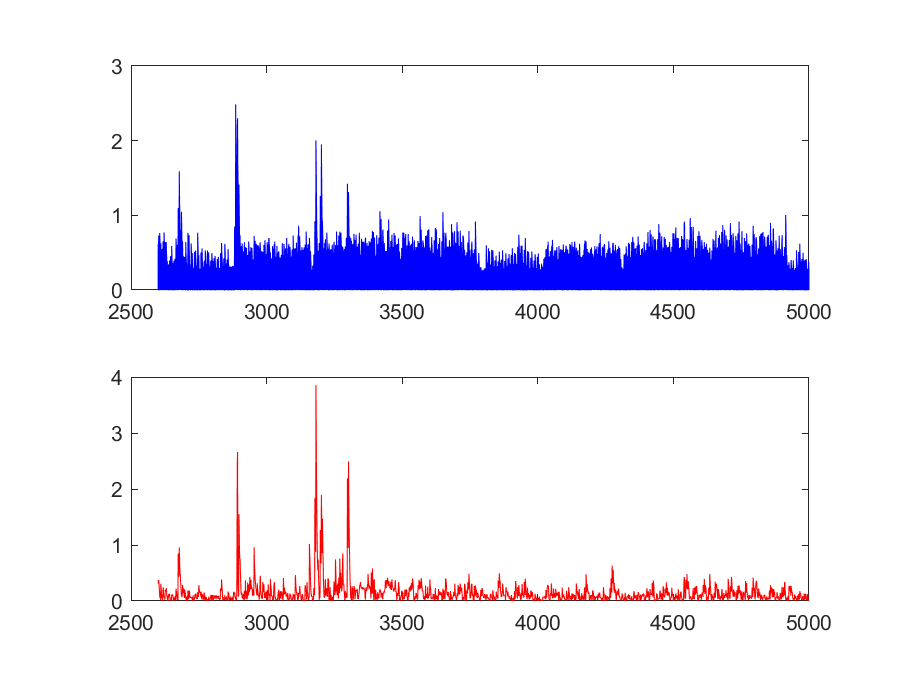
\includegraphics[width=0.8\textwidth]{img/dpa.eps}
    \caption{difference between the two sets for all bad
key guess in blue and for the correct key in red}
    \label{fig:diff_of_means}
\end{figure}
\subsubsection{Why are there other peaks?}
The other peaks could appear for two main reasons:
\begin{enumerate}
    \item correlations due to some linearities that could occur between SBoxs's inputs and outputs
    \item values could be manipulated multiple times
\end{enumerate}

\subsection{Exemplary attack against DES}
Kocher's DPA is a divide and conquer attack.
Increasing the number of rounds doesn't help since it targets the first round.
For perfect security against DPA, the power should be independent with the key.

In Kocher's DPA, we model the noise simply by the value of one bit and the statistical test is a difference of mean.

To recover the whole keys we do the same attack on other bits (divide and conquer).

We only focus on 1 bit considering the others as noise. In general it is better to use the 4 bits and thus have a better SNR. With parallel computation it is harder to attack because there is more noise.

There are several peak because the S-box is not perfect
so if we have good correlation at the input, it's the same at the output.
The higher peak is the correct candidate,
other hight peaks are other values with very close hamming weight.
\subsection{Correlation power Analysis}
This is quite similar to the DPA, but instead, we'll rather use another model and statistical test. The statistical test used here is the Pearson's correlation, based on the leakage and an Hamming weight Leakage Model.

\[ r_{L_i,M_i} = \frac{\E(L_i, M_i(k) -  \E(L_i) \cdot \E(M_i(k))}{\sigma(L_i) \cdot \sigma(M_i(k)} \]

When the correlation is computed for all the key candidates of each plaintexts, we can select the key that leads to the most correlation.

\[ \hat{k} = \argmax_{k^*} \frac{\E(L_i, M_i^{k^*}) -  \E(L_i) \cdot \E(M_i^{k^*})}{\sigma(L_i) \cdot \sigma(M_i^{k^*})} \]


\subsection{Template Attack with Gaussian distribution (multivariate)}
To execute a Template attack, the attacker must have a similar device in order to preprocess a huge amount of plaintexts to build the models (the templates)
\subsubsection{Finding the point of interest}
First, the attacker needs to find a point of interest where we have a maximum amount of information;
for instance, using the Pearson's correlation or a t-test (like LSB) model, we choose the points that gave us the maximum correlation.

\subsubsection{Profiling}
The first step consists on preparing the leakage model. We assume Gaussian additive noise:
\[
  N(R(L_i) \mid \mu_{v_i}, \sigma_{v_i}) = \frac{1}{2\pi\sqrt{\sigma_{v_i}}} \exp\left(-\frac{1}{2}\left(\frac{(R(L_i)-\mu_{v_i})^2}{\sigma_{v_i}}\right)^2\right).
\]
Here, $v_i$ are each possible values at the output of the S-box (ex: 256 values, each corresponding to one of the 256 possible keys),
while $R(L_i)$ is a measured value of the leakage for the corresponding output value $v_i$.
$\mu_{v_i}$ and $\sigma_{v_i}$ are estimated based on the leakages with the value $v_i$.

For each byte of key, we will have 256 templates with 256 pairs $(\mu_i,\sigma_i)$.

\subsubsection{Online}
We can recover the key by selecting
\[
  \hat{k}  = \argmax_{k^*} \prod_{i=1}^q \frac{1}{2\pi\sqrt{\sigma_L}} \exp\left(-\frac{1}{2}\left(\frac{l-m_i^{k^*}}{\sigma_L}\right)^2\right).
\]

\subsection{Improved attacks}
To improve the attack we can:
\begin{itemize}
  \item Improve the measurement setup;
  \item Do an adaptive selection of the inputs;
  \item Do a preprocessing of the traces;
  \item Improve leakage model with profiling, characterization;
  \item Exploit multiple samples, multivariate statistics (e.g. choose $y$ and $z$);
    \begin{itemize}
      \item Higher order attacks;
      \item Template attacks;
    \end{itemize}
  \item Do different statistical tests:
    \begin{itemize}
      \item Difference of mean;
      \item Correlation analyser;
      \item Bayesian classification.
    \end{itemize}
  \item Try to remove the noise, filtering;
  \item Improve the model (Hamming weight) with Profiling, Supervised Machine Learning.
\end{itemize}

For Template Attacks we can use probability and the correct key tends to 1.
Note that for the CPA with Pearson's correlation coefficient we can also have probability with confidence intervals.


\subsection{Countermeasures}
\begin{itemize}
  \item Use a huge table so there is no computation so no dependence on hamming weight;
  \item Huge variance so we need much more samples (SNR).
    Signal is variance of the mean and noise is mean of the variance.
  \item Encoding the data so that they have the same hamming weigth.
\end{itemize}
Note the following about countermeasures
\begin{itemize}
  \item They are never perfect (they only make the attack harder);
  \item They can be implemented at different abstraction levels
    \begin{itemize}
      \item Physical (noise addition),
      \item Technological,
      \item HW/SW design (time/data randomization),
      \item Algorithmic/protocol (key updates).
    \end{itemize}
  \item To balance with implementation cost.
\end{itemize}
Masking and dual-rails are two typical examples of countermeasures.


\subsection{Key independence and weak keys}
Under the assumption that:
\begin{itemize}
  \item Plaintext are uniformly distributed,
  \item $L_t(x_i,k) = f(x_i \xor k) \neq f(x_i;k)$,
\end{itemize}
Are there weak keys?
With an SPA, yes (a key containing only 0's or 1's) but not in DPA.
If we assume an Hamming weight model and we assume that a plaintext of 8 bits is xored with a fixed key (00000000 or 00000001), then passes through an Sbox and gives us the value z.
After reversing the process and getting to the intermediate value that interests us, we'll observe that
\begin{align*}
L_{k=00000000} &= ( \HW(0),\dots, \HW(255)) \\
L_{k=00000001} &= ( \HW(1),\dots, \HW(254))
\end{align*}
as we have 255 different values for the plaintext, so we would have that $ L_{k=0000}$ = $ L_{k=0001}$ but in a different order.

In conclusion, we learn nothing more with a ``wrong key'' with a DPA. This is why we need to measure the leakage of many plaintexts.


\subsection{Asymptotic equivalences}
Under the additional assumption that:
\begin{itemize}
  \item $L_t(x_i,k) = \delta(x_i,k) + n$;
  \item $n \sim \Norm(\mu,\sigma^2)$,
    identical for all $t$
    and independent of manipulated data;
  \item The same models are used by all distinguishers.
\end{itemize}

Suppose we normalize the leakage, i.e. $\E[L] = 0$ and $\sigma_L = 1$.
For the Pearson's Correlation coefficient, we have
\begin{align*}
  \tilde{k}
  & = \argmax_{k^*} \frac{\E[(L - \E[L])(M^{k^*} - \E[M^{k^*}])]}{\sigma_L\sigma_{M^{k^*}}}\\
  & = \argmax_{k^*} \frac{\E[LM^{k^*} - \E[L\E[M^{k^*}]] - \E[\E[L]M^{k^*}] + \E[L]\E[M^{k^*}]}{\sigma_L\sigma_{M^{k^*}}}\\
  & = \argmax_{k^*} \frac{\E[LM^{k^*} - \E[L]\E[M^{k^*}] - \E[L]\E[M^{k^*}] + \E[L]\E[M^{k^*}]}{\sigma_L\sigma_{M^{k^*}}}\\
  & = \argmax_{k^*} \frac{\E[LM^{k^*}] - \E[L]\E[M^{k^*}]}{\sigma_L\sigma_{M^{k^*}}}\\
  & = \argmax_{k^*} \frac{\E[LM^{k^*}]}{\sigma_{M^{k^*}}}\\
  & = \argmax_{k^*} \frac{\E[LM^{k^*}]}{\sqrt{\E[(M^{k^*})^2] - \E[M^{k^*}]^2}}.
\end{align*}
and for the template attack:
\begin{align*}
  \bar{k}  & = \argmax_{k^*} \prod_{i=1}^q \frac{1}{2\pi\sqrt{\sigma_L}} \exp\Big(-\frac{1}{2}\Big(\frac{l-m_i^{k^*}}{\sigma_L}\Big)^2\Big)\\
           & = \argmin_{k^*} \sum_{i=1}^q \Big(\frac{l-m_i^{k^*}}{\sigma_L}\Big)^2\\
           & = \argmin_{k^*} \sum_{i=1}^q l_i^2 - 2l_im_i^{k^*} + (m_i^{k^*})^2\\
           & = \argmin_{k^*} \E[L^2] - 2\E[LM^{k^*}] + \E[M^{k^*}]^2\\
           & = \argmax_{k^*} 2\E[LM^{k^*}] - \E[M^{k^*}]^2\\
           & = \argmax_{k^*} 2\frac{\E[LM^{k^*}]}{\E[M^{k^*}]^2} - 1\\
           & = \argmax_{k^*} \frac{\E[LM^{k^*}]}{\E[M^{k^*}]^2}.
\end{align*}

Asymptotically, $\E[M^{k^*}]$ and $\sigma(M^{k^*})$ are independent of $k^*$.
In the simple case of univariate model, they are asymptotically equivalent.

The model is more important that the comparison.


\subsection{Paper and pencil estimations}

\paragraph{Does correlation have a normal Distribution?}
In theory no: correlation is limited between $-1$ and $1$, so cannot be Gaussian.

But in practice, it is Gaussian.
If $\rho$ is not too high and the device is not trivial to attack, we need a lot of samples.
We need to sum a lot of samples and it will look like a Gaussian distribution (but not perfectly).

\subsubsection{Important lemmas}
\begin{mylem}
Let $X$, $Y$ and $L$ be 3 random variables such that $Y= X+ N_1$ and $ L = Y+N_2$ with $N_1$ and $N_2$ two additive noise random variables.
We have
\begin{equation}
\rho(X,L) = \rho(X,Y) \cdot \rho(Y,L)
\label{eq:l6_lemma_rhorhorho}
\end{equation}
\end{mylem}
\begin{mylem}
The covariance $\rho$ between the sum of $n$ i.i.d. random variables and the sum of the first $m<=n$ is given by
\begin{equation}
\rho = \sqrt{\frac{m}{n}}
\label{eq:l6_lemma_mn}
\end{equation}
\end{mylem}

\subsubsection{Application}
How does the complexity scales? Assuming a Hamming weight model and that $\rho(M_{k^*},L)=0$ for wrong keys.

If we have an 8 bit architecture as reference, a 32 bits architecture will need 4 times more traces to attack.
A 128 bits architecture will need 16 times more traces.
This depends on the leakage model and the two previous lemmas.
\begin{align*}
    L & = \text{Model} + \text{Noise} = M + N \\
    L & = (M_{\text{predicted}} + M_{\text{unpredicted}}) + N
\end{align*}
the noise model comes from the algorithmic noise due to parallel computations, and from physical noise.
We can use the first lemma to compute the correlation for each architecture (8, 32 and 128 bits).

We have \[ \rho(L,M_\text{predicted}) = \underbrace{\rho(M_\text{predicted},M)}_{\text{algorithmic noise}} \cdot \underbrace{\rho(M,L)}_{\text{physical noise}}. \]

The only thing that changes, depending on the architecture, is $\rho(M_\text{predicted},M)$ due to the algorithmic noise.
We can find its value by using the second lemma where the $m$ stands for the bits predicted by an S-box (8 bits each time in this case)
and $n$ represents the total amount of bits manipulated by the architecture (8, 32 or 128).

For each architecture:
\begin{align*}
    \rho_{\text{8bits}}(L,M_\text{predicted})   & = \sqrt{\frac{8}{8}}   \cdot \rho(M,L) = \rho(M,L) \\
    \rho_{\text{32bits}}(L,M_\text{predicted})  & = \sqrt{\frac{8}{32}}  \cdot \rho(M,L) = \sqrt{1/4}  \cdot \rho(M,L) \\
    \rho_{\text{128bits}}(L,M_\text{predicted}) & = \sqrt{\frac{8}{128}} \cdot \rho(M,L) = \sqrt{1/16} \cdot \rho(M,L)
\end{align*}
Using the formula that gives the \# of samples needed to complete the attack (where we square the correlation), we can see where the increase of the number of traces comes from and how much algorithmic noise improves security.

However, algorithmic noise is not a good source of noise: the cost of implementing it is linear, but the security improvements are only linear, and not exponential as we would want in cryptography.

This attack depends on the computational power because the attacker could be able to predict 32 bits at the time instead of 8 bits: algorithmic noise is just noise in the adversary's model.
You can replace it in the above equations to find that the number of traces needed decreases.

If the model is not Hamming weight, then the first lemma cannot be used (because non-additive noise).



% Supprimez pas les espaces entre les sections

\section{Side-channel attacks countermeasures: masking}


To protect against side-channel attacks, countermeasures like noise are not sufficient.
However, a technique named \strong{masking}, also known as data randomization, and inspired by the concepts of shared computations, can amplify the impact of noise to increase the security.

The idea of masking is that instead of manipulating directly sensitive variables $x, y, z,\dots$ (like keys, intermediate signals\dots),
we can instead manipulate and perform computations on multiple variables $x_1, x_2, \dots, x_d, y_1, \dots, y_d, z_1, \dots, z_d, \dots$
that can be combined together to recover the original sensitive variables but that,
taken apart, are mostly random and unrelated to the sensitive variable.

For instance, if $y$ is a sensitive variable, then it can be encoded into $d$ shares such that
\[ y = y_1 \xor y_2 \xor \dots \xor y_d. \]
To construct the shares, we do $y_1, \dots, y_{d-1} \leftarrow \{0,1\}^n$, $d-1$ independent random variables with a uniform distribution, and set $y_d=y \xor y_1\xor\dots\xor y_{d-1}$.
The information about $y$ is kept, but is split between different variables. In practice, it looks like a one-time pad.

Then, we can process each share independently of the others, and hope that for the adversary it will be much more difficult to recover the sensitive variable from the different shares.
But we need to ensure that each share is indeed independently processed, and that shares are not recombined by physics or anything like that.

\paragraph{Probing security}
We define $\epsilon$-probing security as the security of a system for which an adversary $A$ that observes $\epsilon$ intermediate values cannot learn anything about $y$.

An unprotected implementation has $\epsilon=0$.
A $d$-share encoding has ideally $\epsilon=d-1$, as the adversary needs to probe $d$ samples at specific points.


\subsection{Computations on shared data}

A first attempt would be to compute it like this: \[ S(y) = S(y_1) \xor \mathrm{Corr_2}(y_1, y_2) \xor \mathrm{Corr_3}(y_1, y_2, y_3) \dots\]
where $\mathrm{Corr}_{i}$ is a correction term.
The issue is that the correction term must then be implemented as a table of size $(2^n)^d\cdot n = \bigoh(2^{nd})$,
an exponential cost for a maybe exponential gain.
In addition to this, there is a problem of independence of the shares, as they are all merged into the table input.

Computing on shared data is difficult.
To ease this, we decompose the circuit as a combination of linear operations and non-linear operations.
In practice, the non-linear operation that is used is multiplication, i.e. AND.

\paragraph{Linear computation}
If $L(\cdot)$ is linear over $\GF(2)$ or $\GF(2^n)$, and $y=y_1\xor\dots\xor y_d$, then
\[ L(y)=L(y_1\xor \dots \xor y_d) = L(y_1) \xor \dots \xor L(y_d) \]
so we can implement a linear operation on a shared variable by simply applying the linear operation on each share independently.

The overhead is $\bigoh(d)$, linear cost for hopefully exponential gains.

\paragraph{Nonlinear computation: wrong idea}
\label{sec:par:l7_gadget_nonlinear_wrong}
A first proposal is to compute the output share by doing partial products followed by compressions:
\[
\begin{bmatrix} a_1 \\ a_2 \\ a_3 \end{bmatrix} \cdot
\begin{bmatrix} b_1 & b_2 & b_3 \end{bmatrix} =
\begin{bmatrix} a_1b_1 & a_1b_2 & a_1b_3 \\ a_2b_1 & a_2b_2 & a_2b_3 \\ a_3b_1 & a_3b_2 & a_3b_3 \end{bmatrix} =
\begin{bmatrix} c_1 \\ c_2 \\ c_3 \end{bmatrix}.
\]
We can check that $a \cdot b = c = c_1 \xor c_2 \xor c_3$.

The problem with this approach is that after the compression phase, we have $c_i=a_ib_1 \xor\dots\xor a_ib_d = a_i(b_1 \xor\dots\xor b_d)=a_i b$.
If an adversary, with a single probe, discovers that $c_i=1$, then it can be sure that $b=1$ and the sensitive value has been unmasked.
And we cannot resolve this by removing the compression phase, otherwise as the circuit becomes deeper, we will have an exponential number of partial products and shares.

\paragraph{Nonlinear computation: correct idea}
We introduce refreshing by adding some new random masks $r_i$ that change nothing to the computation but protect it:
\[
\begin{bmatrix} a_1b_1 & a_1b_2 & a_1b_3 \\ a_2b_1 & a_2b_2 & a_2b_3 \\ a_3b_1 & a_3b_2 & a_3b_3 \end{bmatrix} +
\begin{bmatrix} 0 & r_1 & r_2 \\ -r_1 & 0 & r_3 \\ -r_2 & -r_3 & 0 \end{bmatrix} =
\begin{bmatrix} c_1 \\ c_2 \\ c_3 \end{bmatrix}.
\]
When we compute the compression, to avoid leaking sensitive values by accidental recombinations, we do it like this:
\[ c_1 = (a_1 b_1 \xor 0) \xor (a_1 b_2 \xor r_1) \xor (a_1 b_3 \xor r_2). \]
In a sense, we encrypt our partial products using a one-time pad with new random variables.

The overhead is $\bigoh(d^2)$: quadratic cost for hopefully exponential gains.

\paragraph{Composability}
The advantage of these constructions is that they are composable: they can be combined in any way without creating weak points (provided we don't use other building blocks).


\subsection{Concrete leakage security by reduction}

We have that probing security implies concrete leakage security.

\begin{mytheo}[Probing security implies concrete leakage security]
\label{thm:l7_masking_reduction}
Assume masking scheme with $d$ shares, and leakage variables $L_i = \delta(Y_i) + \Norm_i$ where $\delta(\cdot)$ is a deterministic part and $\Norm_i$ is a Gaussian additive noise, such that
\begin{itemize}
    \item The shares are sufficiently noisy: $\MI(Y_i; L_{Y_i}) < \frac{c}{d}$ where $c$ is a constant factor.
    \item The leakages of the shares are independent.
\end{itemize}
Then, for a masking scheme with $d$ shares and an adversary using $m$ measurements, we have
\[ \SR_{\A}^{kr}(m) \le 1 - \left( 1 - \MI(Y_i;L_{Y_i})^d \right)^m \] % Si quelqu'un sait d'où vient le kr
\end{mytheo}
The $\frac{1}{d}$ factor comes from the fact that, when we do the partial products of the multiplication, each share $a_i$ or $b_i$ is used in $d$ separate partial products and so is used $d$ times.
Because of this, by averaging the samples, the noise power is divided by $d$ (the variance is divided by $\sqrt{d}$), and as the mutual information is proportional to the inverse of the variance, it is increased by a factor $d$.
Thus, if we increase the number of shares, we must also increase in the same amount the variance of the noise to prevent the mutual information from increasing by averaging.

The independence condition states that leakages for $y_i$ only depend on $y_i$, and don't depend on $y_{j\neq i}$.

The number of samples required by an adversary is:
\begin{equation}
\label{eq:l7_adv_N_samples_MId}
N = \frac{c}{\mathrm{\MI}(Y_i; L_{Y_i})^d} \propto \left(\frac{1}{\MI(Y_i; L_{Y_i})}\right)^d.
\end{equation}
Thus, the mutual information needs to be as low as possible.
Then, $N$ grows exponentially with $d$: polynomial implementation cost, exponential security gain.
Good as side-channel attacks are exponentially powerful.

Informally, masking amplifies the noise power exponentially as long as the noise is sufficiently noisy.

Ensuring sufficient noise:
\begin{itemize}
    \item Algorithmic noise: quite convenient, see the previous lecture.
    \item Physical noise (from transistors, jitter\dots): good but usually increases power consumption.
    \item Decrease the signal/the SNR: ex by using dual-rail architecture.
\end{itemize}

\paragraph{Independence issues}
In some cases, seemingly innocent actions can leak secrets.
Ex: if we have a system with $d=2$ shares with $y=y_1\xor y_2$, then if at some point in the program we store $y_1$ in a register, and later we replace the value in the register with $y_2$, then the power consumption required to change it is proportional to $HD(y_1; y_2)=HW(y_1\xor y_2)=HW(y)$, and we have then $\epsilon=0$.
What happens is that one probe gives access to two wires in case of such a ``recombination''.

Another example is when doing partial values in computations, if there is a glitch, the recombination may be leaked.
Yet another example is coupling.

Note: putting wires next to each other doesn't actually leak recombinations, unless there are quadratic terms involved. (HELP NEEDED)

\paragraph{Statistical intuition}
\begin{figure}
    \centering
        \begin{tikzpicture}
            \begin{groupplot}[
                group style={group size=4 by 1, horizontal sep=1.5cm},
                axis lines=left,
                width=0.25\linewidth,
                xlabel={$L_1$},
                ylabel={$L_2$},
                xtick distance=1, ytick distance=1,
            ]
            \nextgroupplot[sticky options={xmin=0, xmax=1.1, ymin=0, ymax=1.1, axis equal, xlabel={$L_1$}, ylabel={$L_2$}}, title={$Y=0$, serial implem.}]
            \addplot[only marks] coordinates { (0, 0) (1, 1) };
            \nextgroupplot[title={$Y=1$, serial implem.}]
            \addplot[only marks] coordinates { (0, 1) (1, 0) };
            \nextgroupplot[sticky options={xmin=-1, xmax=3.1, ymin=0, ymax=1, xlabel={Leakage sum}, ylabel={pdf}}, title={$Y=0$, parallel implem.}]
            \addplot[domain=-1:3, samples=80] {(exp(-2*x^2) + exp(-2*(x-2)^2))/(sqrt(2*pi))};
            \nextgroupplot[title={$Y=1$, parallel implem.}]
            \addplot[domain=-1:3, samples=80] {2*exp(-2*(x-1)^2)/(sqrt(2*pi))};
            \end{groupplot};
        \end{tikzpicture}
    \caption{Statistical intuition}
    \label{fig:l6_statintuit}
\end{figure}
See figure~\ref{fig:l6_statintuit}. Suppose we want to encode $1$ or $0$ using two shares.
\begin{itemize}
    \item To encode $0$, we have two choices: $(0, 0)$ or $(1, 1)$, equally probable.
    \item To encode $1$, we also have two choices: $(0, 1)$ and $(1, 0)$, equally probable.
\end{itemize}
In both cases, the mean value will be $(0.5, 0.5)$: a first order attack doing averaging will fail to differentiate the two.
So, the adversary is forced to do a second order attack (estimating variances) to distinguish the two distributions, and this is much more sensitive to noise.

With three shares, the adversary needs to estimate a third order moment, and so on.

However, if there is an independence issue, then the mean value of one of the distribution may be slightly shifted;
then, it's easier for the adversary to evaluate the mean (1st order) than the moments, when the noise is sufficiently high.


\subsection{Information theoretic metrics}

Shannon entropy (average amount of information in Z samples):
\[ \H[Z] = -\sum_{z\in Z} \Pr[Z=z] \cdot \log_2 \Pr[Z=z] \]

Conditional entropy (remaining secrecy when there is a leak):
\begin{align*}
\H[Z|L] &= -\sum_{l \in L} \Pr[L=l] \sum_{z \in Z} \Pr[Z=z|L=l] \log_2 \Pr[Z=z|L=l] \\
&= -\sum_{z \in Z} \Pr[z] \sum_{l \in L} \Pr[l|z] \log_2 \Pr[Z=z|L=l]
\end{align*}
The second notation is more convenient as usually the secret $z$ is fixed and we want to generate then all the leakages $l$.

Mutual information (how much was leaked):
\[ \mathrm{MI}(Z; L) = H[Z] - H[Z|L] \]

\paragraph{Noiseless Hamming weight distance example}
Suppose we have a system where $z=S(y)=S(x\xor k)$. Then, with a specific key $k^*$, we can generate a model $m^{k^*}$ for the leakage values, and compare this model with the actual leakage to determine which $k^*$ is the correct key (main principle of DPA).

Here, our model will be that $l=\HW(z)$, with $z$ $n$-bit wide.

Then, in the noiseless case, we can estimate analytically the quantities $\Pr[z, l]$ (joint distribution), $\Pr[l]$, $\Pr[z]$ (marginal prob.), $\Pr[z|l]$, $\Pr[l|z]$ (conditional prob.), and finally $\H[Z|L]$ and $\MI(Z;L)$ (left to the reader).

\paragraph{Noisy Hamming weight example}
Now, if we have noise, the model becomes $l=\HW(z) + \Norm(0, \sigma_n)$. Then, we need to manipulate probability density functions
\[ \Pr[l|z] = f(l|z) = \Norm(l | \HW(z), \sigma_n) \]
and use integrals to compute the entropy:
\[ \H[Z|L] = -\sum_{z} \Pr[z] \int_{l} f(l|z) \log_2 \Pr[z|l] \dif{l}. \]
Estimating the probabilities become much more difficult, and we have to resort to sampling for estimation.

\subsubsection{Application to the DPA}
DPA is a form of known plaintext attack. The mutual information is:
\begin{align*}
\MI(K; X, L) &= \H[K] + \sum_{k} \Pr[k] \sum_{x} \Pr[x|k] \sum_{l} f(l | k, x) \log_2 \Pr[k | x, l] \\
&= \H[K] + \sum_{k} \Pr[k] \sum_{x} \Pr[x] \sum_{l} f(l | k, x) \log_2 \Pr[k | x, l].
\end{align*}

Now, the problem of side-channel attacks is that they rely on \emph{models}, which are approximation of the reality.
In particular, the true $f(l | k, x)$ is unknown, so we have to use approximations:
\[ \PI(K; X, L) = \H[K] + \sum_{k} \Pr[k] \sum_{x} \Pr[x|k] \sum_{l} f_{\text{chip}}(l | k, x) \log_2 \hat{\Pr}_{\text{model}} [k | x, l]. \]
Here, we define the \emph{perceived information} as a mutual information when the model of the chip is different from the reality.

If $\Pr_{\text{chip}} = \hat{\Pr}_{\text{model}}$, then the PI is just the MI.

The perceived information can only be computed by sampling (as $f_\text{chip}$ is unknown).
And, it can be negative, if the models differ too much: an adversary using this model learns nothing.

This may seem like a problem for the adversary and thus, an advantage for the designer, but actually it is the inverse:
if a designer wants to reliably estimate the security of its device, it needs to test for \emph{all} possible models, especially the worst-case adversary (which has the exact $f_\text{chip}$ model):
we need to be extremely good adversaries against ourselves!
The MI is actually computed when we have the strongest Bayesian adversary.
If the models differ too much, the PI is reduced: it gives a false sense of security, as the MI is still the same.

So, in practice, we need to bound the unknown distributions.

The difficulty of estimating the MI, especially if multivariate (leakage of different shares), leads to a difficulty to use the reduction theorem that gives concrete security.

\subsubsection{First Order Simplification}
To simplify a bit the computations, at the first order, we have the following theorem:
\begin{mytheo}
If $X$ and $Y$ are two normally distributed variables with means $\mu_X$ and $\mu_Y$ and variances $\sigma_X^2$ and $\sigma_Y^2$, then:
\begin{align*}
\MI(x,y) &= -\frac{1}{2} \cdot \log_2 \left( 1-\rho(x,y)^2 \right) \\
%& = -\frac{1}{2} \cdot \log_2 \left( 1-\frac{1}{1+\frac{1}{\SNR}} \right) \\
%& \propto \SNR \coloneqq \frac{ \Var_Y(\E(L)) }{ \E_Y(\Var(L)) }
\end{align*}
\end{mytheo}
What this means is that the mutual information behaves more or less as the correlation coefficient, provided that the same leakage model is used.

Of course, this theorem requires that the leakage is Gaussian: for Hamming weights, this is not true, it is rather a Gaussian mixture (see figure~\ref{fig:l7_gaussian_mixture}).
But for sufficiently large noise, this approximation holds.
\begin{figure}
    \centering
    \begin{tikzpicture}[
        declare function={normpdf(\x,\m,\s)=exp(-(\x-\m)^2/(2*\s^2))/(sqrt(2*pi)*\s);}
    ]
        \begin{groupplot}[
            group style={group size=2 by 1, horizontal sep=2cm},
            axis lines=left,
            width=0.4\linewidth,
            xlabel={Leakage value},
            xtick distance=1, ytick distance=0.1,
            xmin=-1, xmax=9,
            ymin=0
        ]
        \nextgroupplot[ylabel={Probability}]
        \addplot+ [ycomb] coordinates {(0, 0.00390625) (1, 0.03125) (2, 0.109375) (3, 0.21875) (4, 0.2734375) (5, 0.21875) (6, 0.109375) (7, 0.03125) (8, 0.00390625)};
        \nextgroupplot[ylabel={Probability density}]
        \addplot[domain=-1:9, samples=150] {0.004*normpdf(x, 0, 0.2) + 0.03*normpdf(x, 1, 0.2) + 0.11*normpdf(x, 2, 0.2) + 0.22*normpdf(x, 3, 0.2) + 0.27*normpdf(x, 4, 0.2) + 0.22*normpdf(x, 5, 0.2) + 0.11*normpdf(x, 6, 0.2) + 0.03*normpdf(x, 7, 0.2) + 0.004*normpdf(x, 8, 0.2)};
        \end{groupplot}
    \end{tikzpicture}
    \caption{Leakage function probability distribution}
    \label{fig:l7_gaussian_mixture}
\end{figure}


\subsection{Paper and pencil estimation}
As an example of what we can do with masking, let's apply the technique to the multiplication chain of the AES S-box used to compute the inverse (figure~\ref{fig:l7_multchain}).

We assume $d=3$ shares, the constant $c = 10$ in equation~\ref{eq:l7_adv_N_samples_MId}, and a $\SNR$ of $10^{-2}$.
The mutual information is related to the SNR as per figure~\ref{fig:l7_pp_mi_snr}.
\begin{figure}[ht]
    \centering
    % Don't hesitate to simplify this diagram...
    \begin{tikzpicture}[
    squaring/.style = {draw, rectangle, thick, minimum width=2em, minimum height=2em},
    mult/.style = {draw, rectangle, thick, minimum width=2em, minimum height=2em},
    sum/.style = {draw, circle, thick, minimum width=2em, minimum height=2em},
    input/.style = {draw},
    >={Stealth[round]},
    every new ->/.style = {shorten >=1pt},
    graphs/every graph/.style = {edges=rounded corners},
    skip loop/.style = {to path={-- ++(0, #1) -| (\tikztotarget)}}
    ]
    \matrix[row sep=2mm, column sep=3mm] {
    & \node (k0) [coordinate] {}; \\
    \node (p0) [coordinate] {};
    & \node (plus) [sum] {$+$}; & \node (p1) [coordinate] {};
    & \node (sq2) [squaring] {$(\cdot)^2$}; & \node (p2) [coordinate] {};
    & \node (m1) [mult] {$\otimes$}; & \node (p3) [coordinate] {};
    & \node (sq4) [squaring] {$(\cdot)^4$}; & \node (p4) [coordinate] {};
    & \node (m2) [mult] {$\otimes$}; & \node (p5) [coordinate] {};
    & \node (sq16) [squaring] {$(\cdot)^{16}$}; & \node (p7) [coordinate] {};
    & \node (m3) [mult] {$\otimes$}; & \node (p8) [coordinate] {};
    & \node (m4) [mult] {$\otimes$}; & \node (p9) [coordinate] {}; \\
    };
    \draw
    (p0) node[left] {$x$}
    (k0) node[above] {$k$}
    (p1) node[above] {$y$}
    (p2) node[above] {$a$}
    (p3) node[above] {$b$}
    (p4) node[above] {$c$}
    (p5) node[above] {$d$}
    (p7) node[above] {$e$}
    (p8) node[above] {$f$}
    (p9) node[right] {$z$};
    \graph[use existing nodes] {
        p0 -> plus -- p1 -> sq2 -- p2 -> m1 -- p3 -> sq4 -- p4 -> m2 -- p5 -> sq16 -- p7 -> m3 -- p8 -> m4 -> p9;
        k0 -> plus;
        p1 ->[skip loop=-8mm] m1;
        p2 ->[skip loop=-12mm] m4;
        p3 ->[skip loop=-8mm] m2;
        p4 ->[skip loop=-10mm] m3;
    };
    \end{tikzpicture}
    \caption{Multiplication chain for the computation of }
    \label{fig:l7_multchain}
\end{figure}
\begin{figure}[ht]
    \centering
    \begin{tikzpicture}
    \begin{axis}[
        axis equal image,
        xlabel={$\log_{10}(\SNR)$},
        ylabel={$\log_{10}(\MI(Y;L))$},
        xtick distance=2, ytick distance=2
    ]
    \addplot[domain=-4:4, samples=30] {ln(sqrt(exp(x)^2/(1+exp(x)^2)))};
    \end{axis}
    \end{tikzpicture}
    \caption{MI in function of SNR}
    \label{fig:l7_pp_mi_snr}
\end{figure}

We observe in the plot of figure~\ref{fig:l7_pp_mi_snr} that $\MI(x,y) \propto \SNR$ and find an MI for one share of $10^{-2}$. But we'll discuss about the difference between these methods:
\begin{enumerate}
    \item Suppose that the adversary can exploit one triple of leakages; this means that
    \[\MI(\text{triple}) = \MI(z; L(z_1), L(z_2), L(z_3))\]
    (the adversary has 3 shares, probed at one place). Then, we have:
    \begin{align*}
        \MI(\text{triple}) &= (10^{-2})^3 \\
        N_{\text{3 shares}} &= \frac{c}{\MI^d} = \frac{10}{(10^{-2})^3} = 10^7
    \end{align*}

    \item Now, suppose the adversary has access to all 8 intermediate values in the multiplicative chain (so, to $y$, $a$, $b$, \dots, $f$ and $z$), and it has 3 triples for each.
    Then, the mutual information for each triple is the same, because each triple has the same amount of noise. Then,
    \begin{align*}
        \MI(\text{1 share}) &= 10^{-2} \\
        \MI(\text{3 shares}) &= (10^{-2})^3 \\
        \MI(\text{all shares}) &= 8 \cdot (10^{-2})^3 \\
        N_{\text{all shares}} &= \frac{10}{8*(10^{-2})^3} = 1.25 \cdot 10^6
    \end{align*}

    \item Now, suppose the adversary exploits all the leakage samples of the secure multiplication matrices (for one variable, ex. $z$), that is, all the partial products.
    Then, we have that
    \[ \MI(\text{all multiplication shares}) = 2 \cdot d \cdot \MI(\text{triple of shares}) \]
    This comes from the fact that if we know $a$ (resp. $b$) in the multiplication, then we have $3$ partial products and thus triples that can give us $b$ (resp. $a$).
    This is linked to paragraph~\ref{sec:par:l7_gadget_nonlinear_wrong}.

    Here, we can find the mutual information for the multiplication's example in the 6.1 section. We have 2 values and 3 shares. This equation comes from the fact that if we know $c_1$, we known $a_1\cdot(b_1+b_2+b_3) = a_1\cdot b$. So we must multiply the MI by the number of shares. The 2 stands for the number of variables because we could have done this for a and for b.

    Replacing values, we have
    \begin{align*}
        \MI(\text{multiplication}) &= 6 \cdot 10^{-6} \\
        \MI(\text{total}) &= \underbrace{4 \cdot (6 \cdot 10^{-6})}_{\text{multiplications, 4 boxes}} + \underbrace{4 \cdot 10^{-6}}_{\text{squarings, 4 boxes}} \\
        &= 28 \cdot 10^{-6} \\
        N_{\text{all partial products}} &= \frac{10}{28\cdot 10^{-6}} = 3.6 \cdot 10^5
    \end{align*}

    \item Now, suppose that the adversary targets a circuit where each share is manipulated twice.
    That means that when it probes one share, he actually probes the same share twice, so that it is averaged.
    Then,
    \begin{align*}
        \MI(\text{1 share}) &= 2 \cdot 10^{-2} \\
        \MI(\text{3 shares}) &= (2 \cdot 10^{-2})^3 = 8 \cdot 10^{-6} \\
        N_{\text{3 shares used twice}} &= \frac{c}{\MI^d} = \frac{10}{8 \cdot 10^{-6}} = 1.25 \cdot 10^6
    \end{align*}
\end{enumerate}

This leads us to the conclusion that probing a share that is used twice gives us better results than probing 8 intermediate values because, by probing twice, we're reducing the noise effects before they'll be amplified by the number of shares. In this example, we also obtain the same value than with 8 intermediates values but if you try this exercise with 4 shares and one intermediate value probed 3 times, you'll see the difference.

Thus, the strongest improvement for the attack that an adversary can have is by using averaging:
probing a share that is used multiple times at the probing time, so that averaging takes place before the mutual information is raised to $d$.

\paragraph{What happens in distance-based leakage?}
Distance-based leakages occur when, e.g., a share $z_2$ overwrites a register that contained the share $z_1$, or when there is a non-independence between the shares.
% WTF is this? Should be better explained
Suppose we have $d$ shares: $z = z_1 \xor \dots \xor z_3$.
Then, if shares $z_i$ and $z_j$ share the same register on different cycles, then we will have a leakage $\propto \HD(z_i,z_j) = \HW(z_i \xor z_j)$.
So, one probe will give information on two shares simultaneously.
And with $\ceil{\frac{d}{2}}$ probes, we will get hopefully sufficient information to recover $z$ entirely.
The scheme is thus $\ceil{\frac{d}{2}}-1$-probing secure instead of $d-1$-probing secure.

Example for $d=3$, we go from $2$-probing secure to $1$-probing secure.
We'll only need to recover $\HD(z_1,z_2)$ and $\HW(z_3)$ to recover $z$.
And in the theorem~\ref{thm:l7_masking_reduction}, we will have $\MI(\text{3 shares}) = (10^{-2})^2$ instead of $(10^{-2})^3$.


\subsection{Leveraging masking}
Because masking is difficult and expensive to implement, it is better to restrict masking to only a sensitive part of the circuit, which generates the keys and secrets that vary every time, and use these keys and secrets in a ``classic'' circuit.

Example: use leakage-resilient modes of operations. For instance, take the secret key $k$ and an initialization vector (a fresh, random value) that is public to generate a fresh key $k_0$ (e.g., use a function $F(k, IV)$ then use this $k_0$ to derive two streams: a first one $(k_{0,0}=k_0, k_{0,1}, k_{0,2},\dots)$ that are created with $k_{0,i+1}=F(k_{0,i}, p_A)$ (with $p_A$ a public ``plaintext'') and $(y_1, y_2, \dots)$ created with $k_{1,i}=F(k_{0,i}, p_B)$ (with $p_B$ another public plaintext), and finally do $c_i=m_I\xor k_{1,i}$.

But this poses a problem to the definition of ``security against leakages''.

Modern techniques: prevent key recovery by ``changing'' the key, use message authentication codes\dots.

% TODO add figure




% Supprimez pas les espaces entre les sections

\section{Fault Attacks}

\paragraph{Discussion link}
\url{http://www.forum-epl.be/viewtopic.php?t=12120}

\subsection{How to introduce a fault}
There are different ways to introduce a fault:
\begin{itemize}
  \item Reduce supply voltage;
  \item Increase clock frequency;
  \item Glitch (IO, clock supply) (useful because localized in time, we see the error propagate);
  \item Increase temperature.
\end{itemize}

Note that with Glitch we can do it at a certain time
but with laser we can do it with a certain time \emph{and} at a certain coordinate.

Focused Ion Beam (FIB)
can cut the circuit layer by layer.
Reverse engineers often have access to it.

What is efficient against fault attacks is rekeying when a fault is detected.

\subsection{Generic fault attacks}
If we can change each bit of the key separately,
we can set all the bits of the key to 0 except one.
Then we look at the ciphertext/plaintext pair
and check with 2 encryption what is the value of the bit we have left unchanged.
It is divide and conquer,
once we have found it we do the same for the other bits.

It is the most precise fault. Its drawbacks are that
\begin{itemize}
  \item for an $n$-bit key, we need $n$ faults;
  \item With a glitch, we can easily toggle a bit but setting a bit to 0 is not easy.
\end{itemize}

\subsection{Attacks against the AES}
If we change the ciphertext, we learn nothing of course.

If we introduce an error before ARK of the last round,
\begin{itemize}
  \item with a random byte error we learn nothing,
    it is like a one-time pad;
  \item with a bit toggle it is like toggling it after xoring the plaintext so we learn nothing;
  \item if we can set bits, we can simply set all bits to 0 and the ciphertext will be the last subkey.
\end{itemize}

Introduction an error before ShiftRows, is the same than before ARK since ShiftRows is just routing.

If we introduce an error before SubBytes, if it is a random byte error the output of SubByte will be a random byte
so it will be like a random byte error before ShiftRows, we learn nothing.
If we introduce an error of only one bit, we know in which byte it is but we do not know which bit,
we can find a byte of the subkey with 2 Ciphertext pairs in error and one Ciphertext without error (same Plaintext).
For each pair, we look at the output byte of the SubByte for which the input byte has a bit in error,
trace the bits after the ShiftRows and find which 8 bits of the key are xored with those 8 bits output of the SubByte.
For each values of those 8 bits (256 possibilities), we xor them with the ciphertext, undo the ShiftRows and SubByte.
We do that both with the Ciphertext in error and for the Ciphertext without error and check if the different between the input
of SubBytes is only one bit. There are exactly 8 values of the 8-bits of the key such that it is the case.

We do that for the other Ciphertext in error, we have again 8 values of the 8-bits of the key that works.
Normally (if we are not very unlucky), only one key is appears in both, we have found 8-bits of the first key!
We can do that for the 16 others bytes of the subkey.
We need $16 \cdot 2 = 32$ faulty ciphertexts.

Introducing an error before the ARK of the round 9 is the same than before SubByte of round 10.

Suppose we do a random byte fault on one byte before MixColumn of round 9.
Let $\delta$ be the random byte fault that is xored.
The column for which appear the fault is $(a,b,c,d)$.
Note that since MixColumn is linear,
\[ \MC(a \xor \delta,b,c,d) = \MC(a,b,c,d) \xor \MC(\delta,0,0,0). \]

Suppose we do not know in which of the four byte of the column it is.
There is $255 \times 4 = 1020$ possible patterns:
$(\delta,0,0,0), (0,\delta,0,0), (0,0,\delta,0), (0,0,0,\delta)$.
It affects 32 bits at the output so we need to try $2^{32}$ keys.

The time complexity has increased from $2^8 \cdot 16$ to $2^{32} \cdot 4$
but now we only need $2 \cdot 4$ faulty ciphertext instead of $2 \cdot 16$.

Also the probability that 2 keys works for both ciphertext is smaller since
$1020/2^{32} < 8/2^8$.

If we do the random byte error before ShiftRows of round 9, SubBytes of round 9 or ARK of round 8 it does not change anything
it it still a random byte error on a single byte before MixColumns of round 9.

If the fault is before MixColumns of round 8, ShiftRows of round 8,
SubBytes of round 8 or ARK of round 7, the situation is even better,
the time complexity is still $2^{32}$ but we now only need 2 faulty ciphertexts.
This is explained by the \figuref{fault}.

\begin{figure}[ht]
  \centering
  \begin{subfigure}[b]{0.3\textwidth}
    \begin{tikzpicture}
      \fill [gray] (3,3) rectangle (4,4);
      \draw[step=1.0,black,very thick] (0,0) grid (4,4);
    \end{tikzpicture}
    \caption{Before MixColumns of round 8.}
  \end{subfigure}
  \begin{subfigure}[b]{0.3\textwidth}
    \begin{tikzpicture}
      \fill [gray] (3,0) rectangle (4,4);
      \draw[step=1.0,black,very thick] (0,0) grid (4,4);
    \end{tikzpicture}
    \caption{After MixColumns of round 8.}
  \end{subfigure}
  \begin{subfigure}[b]{0.3\textwidth}
    \begin{tikzpicture}
      \fill [gray] (3,3) rectangle (4,4);
      \fill [gray] (2,2) rectangle (3,3);
      \fill [gray] (1,1) rectangle (2,2);
      \fill [gray] (0,0) rectangle (1,1);
      \draw[step=1.0,black,very thick] (0,0) grid (4,4);
    \end{tikzpicture}
    \caption{After ShiftRows of round 9. One in each column.}
  \end{subfigure}
  \caption{A random byte fault before MixColumns of round 8.}
  \label{fig:fault}
\end{figure}

We see that on the contrary to slide channels attacks, here we like diffusion.

%
% Sequential logic becomes difficult to do with very small circuits, asynchronious logic is being considered.
% But it is a lot harder to implement.
%
% When switching, there is a small time where the electrons can go through (short circuit) -> it is beta_sc
%
% With very small circuits, physics make inter-device variability
%
% Low cost design needs that the block cipher only have 1 S-box.
% It is good for embedded device.
%
%
%
%
% In space, duplicate circuits and compare.
% But if error is done at comparison?:/


\end{document}
